\title[概率论]{第二十一讲: 随机变量的收敛性}
\author[张鑫{\rm Email: x.zhang.seu@foxmail.com}]{\large 张 鑫}
\institute[东南大学数学学院]{\large \textrm{Email: x.zhang.seu@foxmail.com} \\ \quad  \\
	\large 东南大学 \quad 数学学院 \\
	\vspace{0.3cm}
	%\trc{公共邮箱: \textrm{zy.prob@qq.com}\\
		%\hspace{-1.7cm}  密 \qquad 码: \textrm{seu!prob}}
}
\date{}



{ \setbeamertemplate{footline}{}
	\begin{frame}
		\titlepage
	\end{frame}
}

% \begin{CJK*}{GBK}{song}

	%   \title{简单随机抽样}
	%   \author{林语堂}
	%   \institute{University}
	%   \date{2009-03-31}
	%   \date{}
	%   \begin{frame}
		%     \titlepage
		%   \end{frame}

	%   \begin{frame}
		%     \frametitle{第二章:简单随机抽样}
		%     \tableofcontents
		%   %     You might wish to add the option[pausesections]
		%   \end{frame}

	%   \AtBeginSubsection[]{
		%   \begin{frame}<beamer>
			%     \frametitle{Outline}
			%     \tableofcontents[currentsection,currentsubsection]
			%   \end{frame}
		% }
	%   定义目录页

\section{极限定理}
\subsection{随机变量的收敛性}
\begin{frame}
	\frametitle{随机变量的几种收敛性}
	\begin{itemize}[<+-|alert@+>]
		\item \textcolor{red}{几乎必然收敛:} 如果
		\begin{eqnarray*}
			P(\{\omega:\lim_{n\rightarrow\infty}X_n(\omega)=X(\omega)\})=1,
		\end{eqnarray*} 则称随机变量列 $\{X_n\}$ 几乎必然收敛到 $X$, 记作 $X_n\stackrel{a.e.}{\rightarrow} X$, 或 $X_n\rightarrow X, a.s.$

		\item \textcolor{red}{依概率收敛:} 如果对任意的 $\epsilon>0$ 有
		\begin{eqnarray*}
			\lim_{n\rightarrow\infty}P(|X_n(\omega)-X(\omega)|>\epsilon)=0,
		\end{eqnarray*}
		则称 $X_n$ 依概率收敛到 $X$, 记作 $X_n\stackrel{P}{\rightarrow} X$.
		\item \textcolor{red}{$r$ 阶平均收敛:} 设 $r>0$ 为常数,如果随机变量 $X$ 与 $X_n (n\geq 1)$ 的 $r$ 阶矩皆有限,并且有
		\begin{eqnarray*}
			\lim_{n\rightarrow\infty}E|X_n-X|^r=0,
		\end{eqnarray*}
		则称 $\{X_n\}$ 为 $r$ 阶平均收敛到 $X$, 简称 $r$ 阶收敛,记作 $X_n\stackrel{L^r}{\rightarrow} X$.
	\end{itemize}
\end{frame}

\begin{frame}
	\frametitle{几乎必然收敛的刻划与性质}
	\begin{itemize}[<+-|alert@+>]
		\item 若记 $E:=\{\omega: \lim_{n\rightarrow\infty} X_n (\omega)=X (\omega)\}$, 则
		\begin{eqnarray*}
			E=\cap_{m=1}^\infty\cup_{k=1}^\infty\cap_{n=k}^\infty\{\omega:|X_n(\omega)-X(\omega)|<\dfrac{1}{m}\}\in \mathcal{F};
		\end{eqnarray*}
		\item $X_n\stackrel{a.s.}{\rightarrow} X$ 等价于 $P (E)=1$ 或 $P (\bar{E})=0$;
		\item $X_n\stackrel{a.s.}{\rightarrow} X$ 的充分必要条件是对任意的 $\epsilon>0$ 有
		\begin{eqnarray*}
			\lim_{k\rightarrow\infty}P(\cup_{n=k}^\infty|X_n-X|\geq \epsilon)=0
		\end{eqnarray*}
		\item 若 $X_n\stackrel{a.s.}{\rightarrow} X$, 则 $X_n\stackrel{P}{\rightarrow} X$.

	\end{itemize}

\end{frame}


\begin{frame}
	\frametitle{依概率收敛不能推出几乎必然收敛}
	\begin{exam}
		取 $\Omega=[0,1), \mathcal{F}$ 为区间 $[0,1)$ 上的{\rm Borel} 集类,$P$ 为{\rm Lebesgue} 测度。令
		\begin{eqnarray*}
			X_{11}(\omega)=1; \quad
			X_{21}(\omega)=\left\{
			\begin{array}{ll}
				1, &\omega\in [0,\frac{1}{2}),\\
				0, &\omega\in [\frac{1}{2},1);
			\end{array}
			\right.\quad
			X_{22}(\omega)=\left\{
			\begin{array}{ll}
				1, &\omega\in [\frac{1}{2},1),\\
				0, &\omega\in [0,\frac{1}{2});
			\end{array}
			\right.
		\end{eqnarray*}
		一般地,对每个自然数 $k$, 将 $[0,1)$ 等分为 $k$ 个区间,并取
		\begin{eqnarray*}
			X_{ki}(\omega)=\left\{
			\begin{array}{ll}
				1, &\omega\in [\frac{i-1}{k},\frac{i}{k}),\\
				0, &\mbox{其他},
			\end{array}
			\right. i=1,\cdots, k
		\end{eqnarray*}
		定义
		\begin{eqnarray*}
			Y_1=X_{11}, Y_2=X_{21}, Y_2=X_{22}, Y_3=X_{31}, \cdots
		\end{eqnarray*}
		对于随机变量序列 $Y_n$, 对任意的 $\epsilon>0$ 有
		\begin{eqnarray*}
			P(|X_{ki}(\omega)|\geq \epsilon)\leq \dfrac{1}{k}\rightarrow 0,
		\end{eqnarray*}
		但是收敛的点集 $E=\emptyset$, 即 $Y_n$ 不几乎必然收敛.
	\end{exam}

\end{frame}

\begin{frame}
	\frametitle{$r$ 阶收敛与依概率收敛}
	\begin{lem}
		({\rm Markov} 不等式) 设随机变量 $X$ 的 $r$ 阶矩有限,则对任意 $\epsilon>0$ 有
		\begin{eqnarray*}
			P(|X|\geq  \epsilon)\leq \dfrac{1}{\epsilon^r}E|X|^r
		\end{eqnarray*}

	\end{lem}


	\pause
	\begin{thm}
		若 $X_n\stackrel{L^r}{\rightarrow} X$, 则 $X_n\stackrel{P}{\rightarrow} X$. 反之不真.
	\end{thm}


	\pause

	\begin{exam}
		仍取区间 $(0,1)$ 上的几何概率空间 $(\Omega,\mathcal{F}, P)$. 固定 $r>0$, 令
		\begin{eqnarray*}
			X_n(\omega)=\left\{
			\begin{array}{ll}
				n^{1/r},&\omega\in (0, 1/n),\\
				0, &\omega\in [1/n,1),
			\end{array}
			\right. \quad X(\omega)=0.
		\end{eqnarray*}
		易知 $X_n\stackrel{a.s.}{\rightarrow} X$, 从而 $X_n\stackrel{P}{\rightarrow} X$, 但 $X_n\stackrel{L^r}{\nrightarrow} X$.
	\end{exam}
\end{frame}




\begin{frame}
	\frametitle{依分布收敛 (弱收敛)}
	\begin{defi}
		设随机变量 $X,X_1, X_2,\cdots,$ 的分布函数分别为 $F (x), F_1 (x),F_2 (x),\cdots,$, 如果对 $F (x)$ 的任一连续点 $x$ 均有
		\begin{eqnarray}\label{eq:weakdefn}
			\lim_{n\rightarrow}F_n(x)=F(x),
		\end{eqnarray}
		则称 $\{F_n (x)\}$ 弱收敛于 $F (x)$, 记作 $F_n (x)\stackrel{W}{\rightarrow} F (x)$. 此时也称 $\{X_n\}$ 按分布收敛于 $X$, 记作 $X_n\stackrel{W}{\rightarrow} X$.
	\end{defi}
	\pause
	\begin{rmk}
	后面我们用$C_F$表示函数$F(x)$的连续点集, 即
	\[C_F:=\{x: x\mbox{为}F(x)\mbox{的连续点}  \}\]
	\end{rmk}

\end{frame}

\begin{frame}
	\frametitle{为何要求分布函数在连续点收敛,而不是每一点收敛}
	\begin{exam}
		考虑随机变量序列 $\{X_n\}$ 服从如下退化分布
		\begin{eqnarray*}
			P(X_n=\frac{1}{n})=1, n=1,2,\cdots,
		\end{eqnarray*}
		它们的分布函数分别为 $F_n (x)=\left\{
		\begin{array}{ll}
			0, & x<\frac{1}{n}\\
			1, &x\ge \frac{1}{n}
		\end{array}
		\right.$

		\pause
		\begin{itemize}[<+-|alert@+>]
			\item 则在点点收敛要求下,$\{F_n (x)\}$ 的极限函数为 \pause
			\begin{eqnarray*}
				g(x)=\left\{
				\begin{array}{ll}
					0, & x\le 0\\
					1, &x>0
				\end{array}
				\right.
			\end{eqnarray*}
			\pause 显然上述极限不满足右连续性,即 $g (x)$ 不是一个分布函数.\pause
			\item 因为 $F_n (x)$ 在 $x=1/n$ 处有跳跃,故当 $n\rightarrow\infty$ 时,跳跃点的位置趋于 0,\pause 很自然的认为 $\{F_n (x)\}$ 应该收敛于点 $x=0$ 的退化分布,即 $F (x)=\left\{
			\begin{array}{ll}
				0, & x<0\\
				1, &x\ge 0
			\end{array}
			\right.$. \pause 但是对任意的 $n$, 有 $F_n (0)=0$, 而 $F (0)=1$, 所以 $\lim_{n\rightarrow\infty} F_n (0)=0\neq 1=F (0)$, 而这个不收敛的点恰为 $F (x)$ 的不连续点.
		\end{itemize}
	\end{exam}
\end{frame}
\begin{frame}
	\frametitle{依概率收敛与依分布收敛的关系}
	\begin{thm}
		若 $X_n\stackrel{P}{\rightarrow} X$, 则 $X_n\stackrel{W}{\rightarrow} X$.
	\end{thm}

	\pause \zheng 设随机变量 $X,X_1, X_2,\cdots,$ 的分布函数分别为 $F (x), F_1 (x),F_2 (x),\cdots,$ \pause 只需证在 $F (x)$ 的连续点上均有 $F_n (x)\rightarrow F (x)$ 即可. \pause 而要证明这一点我们只需要说明,对任意的 $x$ 均有
	\begin{eqnarray*}
		F(x-0)\le \liminf_{n\rightarrow\infty} F_n(x)\le \limsup_{n\rightarrow\infty} F_n(x)\le F(x+0)
	\end{eqnarray*}
	\pause 注意到,对任意的 $x'<x$,
	\begin{eqnarray*}
		\{X\le x'\}&=&\{X_n\le x, X\le x'\}\cup\{X_n>x,X\le x'\}\\
		\pause &\subset&\{X_n\le x\}\cup\{|X_n-X|\ge x-x'\}
	\end{eqnarray*}
	\pause 从而有 $F (x')\le F_n (x)+P (|X_n-X|\ge x-x')$. \pause 再由 $X_n\stackrel{P}{\rightarrow} X$ 知
	\pause \begin{eqnarray*}
		F(x')\le \liminf_{n\rightarrow\infty}F_n(x) \pause \Rightarrow F(x-0)\le \liminf_{n\rightarrow\infty}F_n(x)
	\end{eqnarray*}
	\pause 类似可证,当 $x''>x$ 时,$\limsup_{n\rightarrow\infty} F_n (x)\le F (x+0)$.
\end{frame}
\begin{frame}
	\frametitle{依分布收敛无法推出依概率收敛}
	\begin{exam}
		设随机变量 $X$ 的分布列为
		\begin{eqnarray*}
			P(X=-1)=P(X=1)=1/2
		\end{eqnarray*}
		令 $X_n=-X$, 则 $X_n$ 与 $X$ 同分布,即 $X_n$ 与 $X$ 有相同的分布,故 $X_n\stackrel{W}{\rightarrow} X$, \pause 但对任意的 $\epsilon\in (0,2)$,\pause
		\begin{eqnarray*}
			P(|X_n-X|\ge \epsilon)=\pause P(2|X|\ge \epsilon)=1\nrightarrow 0
		\end{eqnarray*}

	\end{exam}

\end{frame}

\begin{frame}
	\frametitle{若 $X_n$ 依分布收敛至常数 $c$, 则 $X_n$ 概率收敛至常数 $c$}
	\begin{thm}
		若 $c$ 为常数,则 $X_n\stackrel{P}{\rightarrow} c\Leftrightarrow X_n\stackrel{W}{\rightarrow} c$
	\end{thm}

	\pause 只需证明充分性即可。记 $X_n$ 的分布函数为 $F_n (x), n=1,2,\cdots, $ 常数 $c$ 的分布函数为 $F (x)=\left\{
	\begin{array}{ll}
		0, &x<c,\\
		1, &x\ge c.
	\end{array}\right.
	$\pause 故对任意的 $\epsilon>0$,
	\begin{eqnarray*}
		P(|X_n-c|\ge \epsilon)&=&\pause P(X_n\ge c+\epsilon)+P(X_n\le c-\epsilon)\\
		&\le&\pause  P(X_n> c+\epsilon/2)+P(X_n\le c-\epsilon)\\
		&=&\pause 1-F_n(c+\epsilon/2)+F_n(c-\epsilon)\\
		&\rightarrow& \pause 1-F(c+\epsilon/2)+F(c-\epsilon)=0
	\end{eqnarray*}
	\pause 从而 $X_n\stackrel{P}{\rightarrow} c$.
\end{frame}


\begin{frame}
	\frametitle{弱收敛的充分条件}
	\begin{thm}
		设 $F (x), F_n (x)(n\geq 1)$ 均为分布函数,如果对于 $F(x)$的连续点集$C_F$ 的某个稠密子集 $D$ 上的一切 $x$ 均有
		\begin{eqnarray}\label{eq:wchou}
			\lim_{n\rightarrow\infty}F_n(x)=F(x), \forall x\in D
		\end{eqnarray}
		则 $F_n\stackrel{W}\rightarrow F$.
	\end{thm}
\pause

\zheng 由 $D \subset C_{F}$ 立得必要性.下设\eqref{eq:wchou}式成立. 对任何 $x \in C_{F}$,取
$$y<x<z \text{且} y, z \in D,$$ 则有\pause
\begin{align}
	F_{n}(y) \leq F_{n}(x) \leq F_{n}(z).
\end{align}\pause
上式令 $n \rightarrow \infty$并利用\eqref{eq:wchou}式可得
\[
F(y)=\lim _{n} F_{n}(y) \leq \varliminf_{n} F_{n}(x) \leq \varlimsup_{n} F_{n}(x) \leq \lim _{n} F_{n}(z)=F(z) .
\]
\pause
再令 $y \uparrow x$ 及 $z \downarrow x$ 便得证\eqref{eq:weakdefn}式. 即 $F_{n} \xrightarrow{W} F$ 。证毕。


\end{frame}
%\subsection{弱收敛与特征函数列收敛的等价性}


\begin{frame}
	\frametitle{{\rm Helly} 第一定理}
	\begin{thm}
		({\rm Helly} 第一定理)任意分布函数列 $F_n(x)$ 均存在子列$F_{n(k)}(x)$以及一个有界、非降、右连续的函数$F(x)$使得对任意的$x\in C_F$, 均有
		\[\lim _{k \rightarrow \infty} F_{n(k)}(x)=F(x).\]  %弱收敛于某个有界,非降且右连续函数的子序列.
	\end{thm}\pause
\begin{rmk}
极限函数 $F(x)$ 不一定为分布函数. \pause 比如, 若$a+b+c=1$, $G(x)$为分布函数, 令$F_{n}(x)=a 1_{(x \geq n)}+b 1_{(x \geq-n)}+c G(x)$, 则易知\begin{pauses}
	\[F_{n}(x) \rightarrow F(x)=b+c G(x),\]\pause
	但
	\[\lim _{x \downarrow-\infty} F(x)=b\neq 0, \quad  \lim _{x \uparrow \infty} F(x)=b+c=1-a\neq 1\]
\end{pauses}
\end{rmk}



\end{frame}


\begin{frame}
	\frametitle{{\rm Helly} 第一定理证明}


\begin{itemize}[<+-|alert@+>]
	\item 令 \( q_{1}, q_{2}, \ldots \) 为有理数排列, \(m_{0}(j) \equiv j\). 由于对每个$k$, \[  F_{m}\left(q_{k}\right) \in[0,1], \quad \forall m\geq 1.\]
	\pause 因此, 存在\( m_{k-1}(j)\)的子列\( m_{k}(j) \)使得\pause
	\[
	\lim_{j \rightarrow \infty}F_{m_{k}(j)}(q_{k}) = G(q_{k}).
	\]
\item 令 $F_{n(k)}(x):=F_{m_k(k)}(x)$, 则 \pause
\[\lim_{k \rightarrow \infty}F_{n(k)}(q) = G(q),\quad  \forall q \in \mathbb{Q}.\]
	\item 令\( F(x)=\inf \{G(q): q \in \mathbb{Q}, q>x\} \), 则易知$F(x)$右连续. \pause 事实上,
	\[
	\begin{aligned}
	\lim _{x_{n} \downarrow x} F\left(x_{n}\right) & =\pause \inf \left\{G(q): q \in \mathbb{Q}, q>x_{n} \text { 对某个 } n\right\} \\
	& =\pause \inf \{G(q): q \in \mathbb{Q}, q>x\}=\pause F(x)
	\end{aligned}
	\]

	\end{itemize}
\end{frame}

\begin{frame}
	\frametitle{{\rm Helly} 第一定理证明II}


\begin{itemize}[<+-|alert@+>]

\item 右连续性证明方法2:对任何 $\varepsilon>0$, 总存在 $q_{k}>x$ 使 $G\left(q_{k}\right)<F(x)+\varepsilon$, 且对于一切 $y \in\left(x, q_{k}\right)$ 有
\[
F(x)\leq F(y)<G\left(q_{k}\right)<F(x)+\varepsilon .
\]
先令 $y \downarrow x$ ,再令 $\varepsilon \downarrow 0$ 得 $F(x)\leq F(x+0) \leq F(x)$. 右连续得证.
\item 令$x\in C_F$并取$r_1,r_2,r_3\in\mathbb{Q}$使得$r_{1}<r_{2}<x<r_3$, 则
	\[
	F(x)-\epsilon<F\left(r_{1}\right) \leq F\left(r_{2}\right) \leq F(x) \leq F(r_3)<F(x)+\epsilon
	\]
\item 由于
 \[ F_{n(k)}\left(r_{2}\right) \rightarrow G\left(r_{2}\right) \geq F\left(r_{1}\right), \quad  F_{n(k)}(r_3) \rightarrow G(r_3) \leq F(r_3), \]
 \pause 因此, 当$k$充分大时,
	\[
	F(x)-\epsilon<F_{n(k)}\left(r_{2}\right) \leq F_{n(k)}(x) \leq F_{n(k)}(r_3)<F(x)+\epsilon
	\]
	\item 综上可知
	\[\lim_{k \rightarrow \infty}F_{n(k)}(x) = F(x), \quad x\in C_F.\]
\end{itemize}
\end{frame}



\begin{frame}{胎紧(tight)}
	\vspace{-0.1cm}

	\begin{defi}设随机变量$X_n$的分布函数为$F_n(x)$, 我们称分布函数列$\{F_n(x)\}_{n\geq 1}$为胎紧的(tight), 如果对任意的$\epsilon>0$, 存$M_{\epsilon}$使得
	  \[\sup_{n\geq 1}P(|X_n|>M_{\epsilon})\leq\epsilon.\]
	\end{defi}
	\pause%
	\begin{thm}
		分布函数列$\{F_n(x)\}_{n\geq 1}$是胎紧的(tight)的当且仅当对任意的$\epsilon>0$, 存$M_{\epsilon}$使得$\sup_{n\geq 1} \big(1-F_{n}\left(M_{\epsilon}\right)+F_{n}\left(-M_{\epsilon}\right) \big)\leq \epsilon$.
	\end{thm}

	\zheng 充分性, 若$\sup_{n\geq 1} \big(1-F_{n}\left(M_{\epsilon}\right)+F_{n}\left(-M_{\epsilon}\right) \big)\leq \epsilon$, 则由
	{\small \begin{align*}
		\sup_{n\geq 1}P(|X_n|>M_{\epsilon})&=\sup_{n\geq 1}\big(1-F_n(M_{\epsilon})+P(X_n<M_{\epsilon})\big)\\
		&\leq \sup_{n\geq 1}\big(1-F_{n}\left(M_{\epsilon}\right)+F_{n}\left(-M_{\epsilon}\right)\big)\leq \epsilon
	\end{align*}}
	知分布函数列$\{F_n(x)\}_{n\geq 1}$是胎紧的.\pause  反之, 取$K_\epsilon=M_\epsilon+\delta, \delta>0$, 则
	{\small \begin{align*}
		\sup_{n\geq 1}\big(1-F_{n}\left(K_{\epsilon}\right)+F_{n}\left(-K_{\epsilon}\right)\big)&\leq \sup_{n\geq 1}\big(1-F_{n}\left(M_{\epsilon}\right)+P(X_n<-M_\epsilon)\big)\\
		&=\sup_{n\geq 1}P(|X_n|>M_{\epsilon})\leq  \epsilon
	\end{align*}}


	\end{frame}
\begin{frame}{胎紧与分布函数列收敛}
\begin{thm}
	分布函数列$\{F_n(x)\}_{n\geq 1}$的子序列收敛到某个分布函数$F(x)$当且仅当$\{F_n(x)\}_{n\geq 1}$是胎紧的.
 \end{thm}\pause

\zheng
\begin{itemize}[<+-|alert@+>]
\item 假设$\{F_n(x)\}_{n\geq 1}$是胎紧的, 且\( F_{n(k)}(x) \rightarrow F(x) \). 下证 $F(x)$为分布函数,\pause  即证: $F(+\infty)-F(-\infty)=1$.
\item 令 $r, s\in C_F$且\( r<-M_{\epsilon}, s>M_{\epsilon} \), 由
\(F_{n}(r) \rightarrow F(r), \ F_{n}(s) \rightarrow F(s) \)
得 \pause %, we have
\[
\begin{aligned}
1-F(s)+F(r)  &=\pause \lim _{k \rightarrow \infty} \big(1-F_{n(k)}(s)+F_{n(k)}(r) \big)\\
& \leq\lim _{k \rightarrow \infty} \sup_{k\geq 1}\big(1-F_{n(k)}(M_{\epsilon})+F_{n(k)}(-M_{\epsilon}) \big)\\
&\leq \pause \sup_{n\geq 1} \big(1-F_{n}\left(M_{\epsilon}\right)+F_{n}\left(-M_{\epsilon}\right)\big) \leq \pause \epsilon
\end{aligned}
\]
\item 令$r\rightarrow-\infty, s\rightarrow\infty$后再令$\epsilon\rightarrow 0$可得$F(+\infty)-F(-\infty)=1$%.由上可得${\lim \sup _{x \rightarrow \infty} 1-F(x)+F(-x) \leq \epsilon}$
\end{itemize}


\end{frame}
\begin{frame}{定理证明续}
	\begin{itemize}[<+-|alert@+>]
	\item 若极限函数是分布函数,下面用反证法证明$\{F_n(x)\}_{n\geq 1}$是胎紧的.
	\item 若$\{F_n(x)\}_{n\geq 1}$不是胎紧的, 则存在$\epsilon>0$以及子列$n(k)$使得对任意的$k$均有 \pause
	\[
		1-F_{n(k)}(k)+F_{n(k)}(-k) \geq \epsilon,
		\]
		\item 由Helly第一定理可知, $\{F_{n(k)}(x)\}_{k\geq 1}$ 存在子列$\{F_{n\left(k_{j}\right)}\}_{j\geq 1}\rightarrow F(x)$
		\item 令$r, s\in C_F$, $r<0<s$, 则
	\begin{align*}
		1-F(s)+F(r)  &=\pause \lim _{j \rightarrow \infty} \big(1-F_{n\left(k_{j}\right)}(s)+F_{n\left(k_{j}\right)}(r)\big)
		 \\
		&\geq \pause \liminf _{j \rightarrow \infty} \big(1-F_{n\left(k_{j}\right)}\left(k_{j}\right)+F_{n\left(k_{j}\right)}\left(-k_{j}\right)\big) \geq \pause \epsilon
	\end{align*}
\item 令$s \rightarrow \infty, r \rightarrow-\infty$可知$F(x)$不是分布函数, 与假设矛盾. %is not the distribution function of a probability measure.
	\end{itemize}

\end{frame}

\begin{frame}
	\frametitle{{\rm Helly} 第二定理}
	\begin{thm}
		({\rm Helly} 第二定理) 设分布函数列 $\{F_n(x)\}$ 弱收敛于分布函数 $F (x)$当且仅当对任何有界连续函数 $g(x)$ 有
		\begin{eqnarray*}
			\int_{\mathbb{R}}g(x)dF_n(x)\rightarrow\int_{\mathbb{R}}g(x)dF(x).
		\end{eqnarray*}
		或等价的\pause
		\[E[g(X_n)]\rightarrow E[g(X)].\]
	\end{thm}

\end{frame}

\begin{frame}
	\frametitle{一个引理}
	\begin{thm}
		若分布函数列 $\{F_n(x)\}_{n\geq 1}$ 弱收敛于分布函数 $F (x)$, 则存在分布函数为$F_n(x)$的随机变量序列$\{Y_n\}_{n\geq 1}$及分布函数为$F(x)$的随机变量$Y$, 使得$Y_n\rightarrow Y, a.s.$.
	\end{thm}\pause

	\zheng %\begin{proof}\ %
		\begin{itemize}[<+-|alert@+>]
		\item 令$\Omega=(0,1), \mathcal{F}=\mathcal{B}((0,1))$, $P$ 为$(0,1)$上的Lebesgue测度.
		\item 令
		\begin{align*}
			&Y_{n}(y)=F_n^{-1}(y):=\sup \{x: F_{n}(x)<y\}\\
			&Y(y)=F^{-1}(y):=\sup \{x: F(x)<y\}\\
			&a_{y}=\sup \{x: F(x)<y\}, \quad b_{y}=\inf \{x: F(x)>y\}\\
			&\Omega_0=\{y:\left(a_{y}, b_{y}\right)=\emptyset\}
		\end{align*}
		 \item  由于$\left(a_{y}, b_{y}\right)$互不相交且每个非空区间均包含不同的有理数, 因此可知 $\Omega-\Omega_0$ 中的元素个数可数, 从而$P(\Omega-\Omega_0)=0$.

		\end{itemize}

	%\end{proof}

\end{frame}


\begin{frame}
	\frametitle{引理证明(续)}
	\begin{itemize}[<+-|alert@+>]

		 \item 下证, 对任意的$y \in \Omega_{0}$, 我们有$F_{n}^{-1}(y) \rightarrow F^{-1}(y)$.
		 \item 首先, 我们有${\liminf _{n \rightarrow \infty} F_{n}^{-1}(y) \geq F^{-1}(y)}$,
		 \begin{itemize}[<+-|alert@+>]
		 \item 令 $x\in C_F$使得$x<F^{-1}(y)$, 则由$y\in \Omega_0$知$F(x)<y$
		 \item 由$x\in C_F$以及$F_n(x)\rightarrow F(x)$可知, 当$n$充分大时, $F_n(x)<y$, 也即 $F_n^{-1}(y)\geq x$
		 \item 令$n\rightarrow\infty$取下极限后再令$x\rightarrow F^{-1}(y)$可得本结果.
		 \end{itemize}
		 \item 其次, 我们可证${\lim \sup _{n \rightarrow \infty} F_{n}^{-1}(y) \leq F^{-1}(y)}$
		 \begin{itemize}[<+-|alert@+>]
			\item 令 $x\in C_F$使得$x>F^{-1}(y)$, 则由$y\in \Omega_0$知$F(x)>y$
			\item 由$x\in C_F$以及$F_n(x)\rightarrow F(x)$可知, 当$n$充分大时, $F_n(x)>y$, 也即 $F_n^{-1}(y)\leq x$
			\item 令$n\rightarrow\infty$取上极限后再令$x\rightarrow F^{-1}(y)$可得本结果.
		 \end{itemize}


		\end{itemize}
\end{frame}


\begin{frame}
	\frametitle{{\rm Helly} 第二定理证明}
	%\zheng
	\begin{itemize}[<+-|alert@+>]
	\item 必要性
	\begin{itemize}[<+-|alert@+>]
		\item 由引理可知, 存在$\{Y_n\}_{n\geq 1}$及$Y$使得$Y_n\rightarrow Y,    a.s.$
		\item 由于$g(x)$是连续函数, 从而$g(Y_n)\rightarrow g(Y), a.s.$
		\item 从而由控制收敛定理可知
		\[E[g(X_n)]=E[g(Y_n)]\rightarrow E[g(Y)]=E[g(X)], \]
		\pause 也即
	   \[\int_{\mathbb{R}}g(x)dF_n(x)\rightarrow\int_{\mathbb{R}}g(x)dF(x).\]
	\end{itemize}

	\end{itemize}



\end{frame}


\begin{frame}
	\frametitle{{\rm Helly} 第二定理证明}
	%\zheng
	\begin{itemize}[<+-|alert@+>]
	\item 充分性
	\begin{itemize}[<+-|alert@+>]
		\item 令\[
			g_{x, \epsilon}(y)=\left\{\begin{array}{ll}
			1 & y \leq x \\
			0 & y \geq x+\epsilon \\
			\text {linear } & x \leq y \leq x+\epsilon
			\end{array}\right.
			\]
		\item 由 $g_{x, \epsilon} $的定义及连续性可知 %\( g_{x, \epsilon}(y)=1 \) 当 \( y \leq x, g_{x, \epsilon} \) 连续且is continuous, and \( g_{x, \epsilon}(y)=0 \) for \( y>x+\epsilon \),
    \begin{align*}
		&\limsup _{n \rightarrow \infty} P\left(X_{n} \leq x\right) \leq  \pause \limsup _{n \rightarrow \infty} E g_{x, \epsilon}\left(X_{n}\right)=\pause E g_{x, \epsilon}\left(X\right) \leq \pause P\left(X \leq x+\epsilon\right) \pause \\
		&\liminf _{n \rightarrow \infty} P\left(X_{n} \leq x\right) \geq \pause \liminf _{n \rightarrow \infty} E g_{x-\epsilon, \epsilon}\left(X_{n}\right)=\pause E g_{x-\epsilon, \epsilon}\left(X\right) \geq \pause P\left(X\leq x-\epsilon\right) \pause
	\end{align*}
	\item 令\( \epsilon \rightarrow 0 \) 可得
	\begin{align*}
		&\lim \sup _{n \rightarrow \infty} P\left(X_{n} \leq x\right) \leq  \pause P\left(X\leq x\right), \pause \\
		&\lim \inf _{n \rightarrow \infty} P\left(X_{n} \leq x\right) \geq  \pause P\left(X<x\right)\stackrel{x\in C_F}{=}P\left(X \leq x\right)\pause
	\end{align*}

	 \item 由上可得, 对任意的$x\in C_F$, 我们有
	 \[\lim _{n\rightarrow \infty} F_{n}(x)=F(x).\]
		\end{itemize}
	\end{itemize}

\end{frame}


\begin{frame}
	\frametitle{连续性定理及证明}

	\begin{thm}
		(连续性定理) 分布函数列 $\{F_n (x)\}$ 弱收敛到分布函数 $F (x)$ 的充分必要条件是:相应的特征函数列 $\{\varphi_n (t)\}$ 逐点收敛到相应的特征函数 $\varphi (t)$.
	\end{thm}
\pause

\zheng

\begin{itemize}[<+-|alert@+>]
\item 必要性显然. \pause 事实上, 由$\cos(tx), \sin(tx)$为有界连续函数以及Helly第二定理可知
\begin{align*}
	\varphi_n(t)&:=\pause \int_{\mathbb{R}}e^{itx}dF_n(x)\pause
	\\
	&=\pause \int_{\mathbb{R}}\cos(tx)dF_n(x)+i\int_{\mathbb{R}}\sin(tx)dF_n(x)\pause
	\\
	&\rightarrow\pause \int_{\mathbb{R}}\cos(tx)dF(x)+i\int_{\mathbb{R}}\sin(tx)dF(x)\pause
	\\
	&=\pause \int_{\mathbb{R}}e^{itx}dF(x)\pause
	=:\varphi(t).
\end{align*}
%\item
\end{itemize}


\end{frame}
\begin{frame}{连续性定理证明(续)}
下证充分性. 先证$\{F_n(x)\}_{n\geq 1}$是胎紧的.
\begin{itemize}[<+-|alert@+>]
\item 注意到
\begin{align*}
	&u^{-1} \int_{-u}^{u}\left(1-\varphi_{n}(t)\right) d t=\pause u^{-1} \int_{-u}^{u}\int_{\mathbb{R}}\left(1-e^{itx}\right)dF_n(x) d t
	\\ &=\pause u^{-1}\int_{\mathbb{R}}\int_{-u}^{u}\left(1-e^{itx}\right)dt dF_n(x)=\pause 2\int_{\mathbb{R}}(1-\frac{\sin ux}{ux})dF_n(x)\\
	&\geq \pause 2 \int_{|x|\geq\frac{2}{u}}(1-\frac{1}{|ux|})dF_n(x)\geq \pause \int_{|x|\geq\frac{2}{u}}dF_n(x)=\pause P(|X_n|\geq \frac{2}{u})\pause
\end{align*}
\item 另一方面,
\begin{align*}
	&\lim_{n\rightarrow\infty}u^{-1} \int_{-u}^{u}\left(1-\varphi_{n}(t)\right) d t=\pause u^{-1} \int_{-u}^{u}\left(1-\varphi(t)\right) d t \stackrel{u\rightarrow 0}{\longrightarrow} \pause 0
\end{align*}

%\end{itemize}

\item 从而
\[P(|X_n|\geq \frac{2}{u})\leq \pause u^{-1} \int_{-u}^{u}\left(1-\varphi_{n}(t)\right) d t \leq \pause 2 \epsilon
\]
\end{itemize}

\end{frame}

\begin{frame}{连续性定理证明(续)}
其次, 证明对任意的有界连续函数$g(x)$均有 $E[g(X_n)]\rightarrow E[g(X)]$. \pause
\begin{itemize}[<+-|alert@+>]
\item 首先注意到, 对于$\{F_n(x)\}_{n\geq 1}$的任一子列$\{F_{n(k)}(x)\}_{k\geq 1}$, 若$F_{n(k)} (x)\stackrel{W}{\rightarrow} F (x)$, 则分布函数$F(x)$的特征函数必为$\varphi(t)$.
\item 由$\{F_n(x)\}_{n\geq 1}$的胎紧性可知, $\{F_n(x)\}_{n\geq 1}$的任一子列$\{F_{n(k)}(x)\}_{k\geq 1}$均存在子列$\{F_{n(k_j)}(x)\}_{j\geq 1}$弱收敛到某个分布函数$F(x)$, 且$F(x)$的特征函数为$\varphi(t)$.

\item 由于$\{F_{n(k_j)}(x)\}_{j\geq 1}$弱收敛到某个分布函数$F(x)$, 故由Helly第二定理可知, 对任意的有界连续函数$g(x)$均有
\[\int g(x)dF_{n(k_j)}(x)\rightarrow \int g(x)dF(x)\]

\item 故综上可知, $\int g(x)dF_{n}(x)$的任一子列$\int g(x)dF_{n(k)}(x)$均存在子列$\int g(x)dF_{n(k_j)}(x)\rightarrow \int g(x)dF(x)$. 从而, $\int g(x)dF_{n}(x)\rightarrow \int g(x)dF(x)$, 即 $$E[g(X_n)]\rightarrow E[g(X)].$$
\end{itemize}

\end{frame}

% \begin{frame}{作业}
% \begin{enumerate}
% 	\item $\text {如果 } X_{n} \xrightarrow{P} X \text {, 且 } X_{n} \xrightarrow{P} Y \text {. 试证: } P(X=Y)=1 \text {. }$
%   \item 如果 $X_{n} \xrightarrow{P} X, Y_{n} \xrightarrow{P} Y$. 试证:
%   (1) $X_{n}+Y_{n} \xrightarrow{P} X+Y$;
%   (2) $X_{n} Y_{n} \xrightarrow{P} X Y$.
%   \item 试证: $X_{n} \xrightarrow{P} X$  的充要条件为: $\lim_{n \rightarrow \infty}E\left(\dfrac{\left|X_{n}-X\right|}{1+\left|X_{n}-X\right|}\right)=0$.
%   \item 设随机变量序列 $\left\{X_{n}\right\}$ 独立同分布, 其密度函数为
%   $$p(x)=\left\{
% 	\begin{array}{ll}
%   e^{-(x-\alpha)}, & x \geqslant \alpha, \\
%   0, & x<\alpha.
%   \end{array} \right.
%   $$



%   令 $Y_{n}=\min \left\{X_{1}, X_{2}, \cdots, X_{n}\right\}$, 试证: $Y_{n} \xrightarrow{P} \alpha$.
% \end{enumerate}

% \end{frame}


\title[概率论]{第二十二讲:大数定律}
\author[张鑫{\rm Email: x.zhang.seu@foxmail.com} ]{\large 张 鑫}
\institute[东南大学数学学院]{\large \textrm{Email: x.zhang.seu@foxmail.com} \\ \quad  \\
	\large 东南大学 \quad 数学学院 \\
	\vspace{0.3cm}
	% \trc{公共邮箱: \textrm{zy.prob@qq.com}\\
		%  \hspace{-1.7cm}  密 \qquad 码: \textrm{seu!prob}}
}
\date{}


{ \setbeamertemplate{footline}{}
	\begin{frame}
		\titlepage
	\end{frame}
}

\subsection{大数定律}
\begin{frame}
	\frametitle{概率及频率}
	\begin{itemize}[<+-|alert@+>]
		\item 记 $S_n$ 为 $n$ 重伯努利试验中事件 $A$ 出现次数,称 $\dfrac{S_n}{n}$ 为事件 $A$ 出现的频率;
		\item 记 $p$ 为一次试验中 $A$ 发生的概率;
		\item 概率是频率的稳定值,何谓稳定值?似乎与频率的极限有关;
		\item 考虑 $|\dfrac{S_n}{n}-p|$, 如果能类似于函数列极限情形即对任意的 $\epsilon>0$, 存在 $N$ 使得当 $n\ge N$ 时
		\begin{eqnarray*}
			|\dfrac{S_n}{n}-p|< \epsilon, \forall \omega\in \Omega.
		\end{eqnarray*}
		\item 但是上述情形无法做到,事实上,对任意的 $\epsilon<1-p$,
		\begin{eqnarray*}
			&& P(|\dfrac{S_n}{n}-p|< \epsilon)\le \pause P(\dfrac{S_n}{n}-p<\epsilon)\le \pause P(\dfrac{S_n}{n}-p<1-p)\\
			&&=\pause P(\frac{S_n}{n}<1)=\pause 1-P(\frac{S_n}{n}=1)=\pause 1-P(X_1=1,\cdots,X_n=1)\\
			&&=\pause 1-p^n<1
		\end{eqnarray*}
	\end{itemize}
\end{frame}
\begin{frame}
	\frametitle{伯努利大数定律}
	\begin{thm}
		设 $S_n$ 为 $n$ 重伯努利试验中事件 $A$ 出现次数,$p$ 为一次试验中 $A$ 发生的概率,则对任意的 $\epsilon>0$, 有
		\begin{eqnarray*}
			\lim_{n\rightarrow\infty} P (|\frac{S_n}{n}-p|<\epsilon)=1, \quad\mbox{或等价的}\quad \lim_{n\rightarrow\infty} P (|\frac{S_n}{n}-p|\ge\epsilon)=0
		\end{eqnarray*}
	\end{thm}
	\pause \zheng 因为 $S_n\sim B (n,p)$, 故 $S_n\sim B (n,p), E (\frac{S_n}{n})=p, D (\frac{S_n}{n})=\frac{p (1-p)}{n}$. \pause 从而由切比雪夫不等式可得
	\begin{eqnarray*}
		1\ge P(|\frac{S_n}{n}-p|<\epsilon)\ge 1-\dfrac{D(\frac{S_n}{n})}{\epsilon^2}=1-\frac{p(1-p)}{n\epsilon^2}\rightarrow 1  \quad n\rightarrow \infty
	\end{eqnarray*}
	\pause 故
	\begin{eqnarray*}
		\lim_{n\rightarrow\infty}P(|\frac{S_n}{n}-p|<\epsilon)=1
	\end{eqnarray*}
\end{frame}

\begin{frame}
	\frametitle{伯努利大数定律的含义}
	\begin{itemize}[<+-|alert@+>]
		\item 随着 $n$ 的增大,事件 $A$ 发生的频率 $\dfrac{S_n}{n}$ 与其概率 $p$ 的偏差大于预先给定的精度 $\epsilon$ 的可能性越来越小,要多小有多小,这便是频率稳定于概率的含义;
		\item 事实上,由切比雪夫不等式可得
		\begin{eqnarray*}
			P(|\frac{S_n}{n}-p|\ge\epsilon)\le \dfrac{D(\frac{S_n}{n})}{\epsilon^2}=\frac{p(1-p)}{\epsilon^2}\dfrac{1}{n}
		\end{eqnarray*}

		\item 伯努利大数定律提供了用频率来确定概率的理论依据;
		\item 比如要估计某种产品的不合格品率 $p$, 则可从该种产品中随机抽取 $n$ 件,当 $n$ 很大时,这 $n$ 件产品中的不合格品的比例可作为不合格品率 $p$ 的估计值.
	\end{itemize}
\end{frame}
\begin{frame}
	\frametitle{伯努利大数定律的另一形式}
	\begin{itemize}[<+-|alert@+>]
		\item 注意到,在伯努利大数定律中,如果记 $X_i=\bigg\{
		\begin{array}{ll}
			1,& \mbox{第} i\mbox{试验} A\mbox{发生}\\
			0,& \mbox{第} i\mbox{试验} A\mbox{不发生}
		\end{array}
		$, 则 $S_n=\sum_{i=1}^nX_i$, 并且
		\begin{eqnarray*}
			\frac{S_n}{n}=\frac{1}{n}\sum_{i=1}^nX_i, \pause p=E(\frac{1}{n}\sum_{i=1}^nX_i)=\frac{1}{n}\sum_{i=1}^nE(X_i)
		\end{eqnarray*}
		\item 伯努利大数定律的结论为:对任意的 $\epsilon>0$, 有
		\begin{eqnarray*}
			\lim_{n\rightarrow\infty}P(|\frac{1}{n}\sum_{i=1}^n[X_i-E(X_i)]|<\epsilon)=1
		\end{eqnarray*}
		也即
		\begin{eqnarray*}
			\frac{1}{n}\sum_{i=1}^n[X_i-E(X_i)]\stackrel{P}{\rightarrow}0
		\end{eqnarray*}

	\end{itemize}

\end{frame}
\begin{frame}
	\frametitle{(强) 大数定律的一般形式}
	\begin{defi}
		设有一随机变量序列 $\{X_n\}$, 如果对任意的 $\epsilon>0$, 有
		\begin{eqnarray*}
			\lim_{n\rightarrow\infty} P (|\frac{1}{n}\sum_{i=1}^n [X_i-E (X_i)]|<\epsilon)=1 \mbox{ 即 }  \frac{1}{n}\sum_{i=1}^n [X_i-E (X_i)]\stackrel{P}{\rightarrow} 0
			%  \lim_{n\rightarrow\infty}P(|\frac{1}{n}\sum_{i=1}^nX_i-\frac{1}{n}\sum_{i=1}^nE(X_i)|<\epsilon)=1
		\end{eqnarray*}
		则称该随机变量序列 $\{X_n\}$ 满足大数定律。如果进一步有
		\begin{eqnarray*}
			\frac{1}{n}\sum_{i=1}^n[X_i-E(X_i)]\stackrel{a.s.}{\rightarrow}0
		\end{eqnarray*}
		则称 $\{X_n\}$ 满足强大数定律.
	\end{defi}
\end{frame}
\begin{frame}
	\frametitle{切比雪夫大数定律}
	\begin{thm}
		设 $\{X_n\}$ 为一列两两不相关的随机变量序列,若每个 $X_i$ 的方差存在且有共同的上界 $M$, 即 $D (X_i)\le M, \forall i\in \mathbb{N}$, 则 $\{X_n\}$ 服从大数定律,即对任意的 $\epsilon>0$, 有
		\begin{eqnarray*}
			\lim_{n\rightarrow\infty}P(|\frac{1}{n}\sum_{i=1}^nX_i-\frac{1}{n}\sum_{i=1}^nE(X_i)|<\epsilon)=1
		\end{eqnarray*}
		特别的,若 $\{X_n\}$ 独立同分布,且 $D (X_n)<\infty$, 则 $\{X_n\}$ 服从大数定律.
	\end{thm}

	\pause \zheng 注意到
	\begin{eqnarray*}
		P(|\frac{1}{n}\sum_{i=1}^nX_i-\frac{1}{n}\sum_{i=1}^nE(X_i)|\ge\epsilon)&\le&\pause  \dfrac{D(\frac{1}{n}\sum_{i=1}^nX_i)}{\epsilon^2}\\
		&=&\pause \dfrac{1}{\epsilon^2}\dfrac{1}{n^2}\sum_{i=1}^nD(X_i)\\
		&\le&\pause \dfrac{1}{\epsilon^2}\dfrac{M}{n}\rightarrow\pause 0
	\end{eqnarray*}

\end{frame}

\begin{frame}
	\frametitle{马尔科夫大数定律}
	\begin{thm}
		设随机变量序列 $\{X_n\}$ 满足如下马尔科夫条件
		\begin{eqnarray*}
			\dfrac{1}{n^2}D(\sum_{i=1}^nX_i)\rightarrow 0
		\end{eqnarray*}
		则 $\{X_n\}$ 服从大数定律,即对任意的 $\epsilon>0$, 有
		\begin{eqnarray*}
			\lim_{n\rightarrow\infty}P(|\frac{1}{n}\sum_{i=1}^nX_i-\frac{1}{n}\sum_{i=1}^nE(X_i)|<\epsilon)=1
		\end{eqnarray*}
	\end{thm}
\end{frame}
\begin{frame}
	\frametitle{辛钦大数定律}
	\begin{thm}
		设 $\{X_n\}$ 为一列独立同分布随机变量序列,若每个 $X_i$ 的期望存在,则 $\{X_n\}$ 服从大数定律,即对任意的 $\epsilon>0$, 有
		\begin{eqnarray*}
			\lim_{n\rightarrow\infty}P(|\frac{1}{n}\sum_{i=1}^nX_i-\frac{1}{n}\sum_{i=1}^nE(X_i)|<\epsilon)=1.
		\end{eqnarray*}
		特别的,如果 $E|X_i|^k, k=1,2,\cdots$, 存在,则 $\{X_n^k\}$ 服从大数定律.
	\end{thm}

	\pause%
	\zheng 设 $\{X_n\}$ 独立同分布,且 $E (X_i)=a, i=1,\cdots,$, 则只需要证明
	\begin{eqnarray*}
		Y_n:=\dfrac{1}{n}\sum_{i=1}^nX_i\xlongrightarrow{P}a, \quad n\rightarrow \infty
	\end{eqnarray*}
	\pause 由依概率收敛的性质,仅需证 $\varphi_{Y_n}(t)\rightarrow e^{iat}$ 即可。事实上,由
	\pause \begin{eqnarray*}
		\varphi_{Y_n}(t)\pause &=&[\varphi(\frac{t}{n})]^n\pause =[1+\varphi'(0)\frac{t}{n}+o(\frac{t}{n})]^n\pause =[1+ia\frac{t}{n}+o(\frac{t}{n})]^n\\
		&=&\pause \exp\{\dfrac{\ln (1+ia\frac{t}{n}+o(\frac{t}{n}))}{1/n}\}\pause \rightarrow e^{iat}
	\end{eqnarray*}

\end{frame}

\begin{frame}
	\frametitle{Borel-Cantelli引理}
	\begin{thm}
	  对于事件列$\{A_j\}$,有
	  \begin{itemize}[<+-|alert@+>]
	  \item 若$\sum_{n=1}^\infty P(A_n)<\infty$,则
	  \[P(\limsup_{n\rightarrow\infty}A_n)=\lim_{k\rightarrow\infty}P(\cup_{n=k}^\infty A_n)=0\]
	  \item 若$\{A_n\}$相互独立,则$\sum_{n=1}^\infty P(A_n)=\infty$当且仅当
	  \[P(\limsup_{n\rightarrow\infty}A_n)=\lim_{k\rightarrow\infty}P(\cup_{n=k}^\infty A_n)=1\]
	  \end{itemize}
	\end{thm}\pause
	\zheng 1. 注意到$\lim_{k\rightarrow\infty}P(\cup_{n=k}^\infty A_n)\le \pause \lim_{k\rightarrow\infty}\sum_{n=k}^\infty P(A_n)\pause =0.$

	\pause
	2. 由于\pause
	\begin{eqnarray*}
	  P(\cup_{n=k}^\infty A_n)&=&\pause \lim_{m\rightarrow\infty}P(\cup_{n=k}^m A_n)=\pause \lim_{m\rightarrow\infty}(1-P(\cap_{n=k}^m\overline{A}_n))\\\pause
	  P(\cap_{n=k}^m\overline{A}_n)&=&\pause \Pi_{n=k}^m P(\overline{A}_n)=\Pi_{n=k}^m(1-P(A_n))\\
	  &\le&\pause \Pi_{n=k}^m \exp(-P(A_n))=\exp(-\sum_{n=k}^m P(A_n))\pause \stackrel{m\rightarrow\infty}{\longrightarrow} 0
	\end{eqnarray*}

  \end{frame}

\begin{frame}
	\frametitle{{\rm Borel} 强大数定律律}
	\begin{thm}({\rm Borel} 强大数定律)
		设 $S_n$ 为 $n$ 重伯努利试验中事件 $A$ 出现次数,$p$ 为一次试验中 $A$ 发生的概率,则
		\begin{eqnarray*}
			\dfrac{S_n}{n}\stackrel{a.s.}{\rightarrow} p
		\end{eqnarray*}
	\end{thm}

\pause

\fenxi 记${A_{n}=\left\{\left|S_n / n-p\right| \geq \varepsilon\right\}}$, 则定理中的几乎必然收敛的充分必要条件是\pause %由定理 1.1 知, (2.16) 式成立的充分必要条件是
\[
P\left(\limsup_{n} A_{n}\right)=0.
\]

再Borel-Cantelli引理可知, 只需证明\pause
\[
\sum_{n=1}^{\infty} P\left(A_{n}\right)<+\infty.
\]

\pause
若像证明弱大数定律那样用切贝谢夫不等式,我们只能得到
\[
P\left(A_{n}\right) \leq \frac{1}{\varepsilon^{2}} D\left(\frac{S_n}{n}\right)=\frac{p q}{n \varepsilon^{2}} \leq \frac{1}{4 n \varepsilon^{2}} .
\]

\end{frame}

\begin{frame}{Borel 强大数定律证明}
\begin{itemize}[<+-|alert@+>]
\item 用${r=4}$时的马尔科夫不等式可得$P\left(A_{n}\right) \leq \dfrac{1}{\varepsilon^{4}} E\left|\frac{S_n}{n}-p\right|^{4}.$
\item 将${S_n}$写为${n}$个独立伯努利分布随机变量之和${S_n=\sum_{k=1}^{n} X_{k}}$, 从而
\[
E\left[\left|\frac{S_n}{n}-p\right|^{4}\right]=\frac{1}{n^{4}} \sum_{1 \leq i, j, k, l \leq n} E\left[\left(X_{i}-p\right)\left(X_{j}-p\right)\left(X_{k}-p\right)\left(X_{l}-p\right)\right] .
\]
\item 注意${X_{1}, \cdots, X_{n}}$相互独立,故上式和号中仅有
\begin{align*}
	&E\left[\left(X_{i}-p\right)^{4}\right]=p q\left(p^{3}+q^{3}\right)\neq 0,\\
	  &E\left[\left(X_{i}-p\right)^{2}\left(X_{j}-p\right)^{2}\right]=p^{2} q^{2}\neq 0, (i \neq j).
\end{align*}
\item 注意到前者共${n}$项,后者共$ C_n^2C_4^2=3 n(n-1)$项,故我们有%可得到
\[
E\left[\left|\frac{S_n}{n}-p\right|^{4} =\frac{p q}{n^{4}}\left[n\left(p^{3}+q^{3}\right)+3 p q\left(n^{2}-n\right)\right]<\frac{1}{4 n^{2}} .\right.
\]
\item 代入马等科夫不等式右方可得$P\left(A_{n}\right) \leq \dfrac{1}{4 n^{2} \varepsilon^{4}}$, 定理得证.

\end{itemize}
\end{frame}


\begin{frame}{Borel强大数定律的备注}
  \begin{rmk}
	\begin{itemize}[<+-|alert@+>]
	\item 上述定理证明,本质上只用到独立同分布序列的四阶中心矩
	${E\left[\left(X_{k}-p\right)^{4}\right]}$以及${E\left[\left(X_{k}-p\right)^{2}\left(X_{j}-p\right)^{2}\right]}$有限, 并没有用到伯努利情形的其它特性. 所以,在四阶中心矩有限的前提下,其证明可以照搬到一般独立同分布情形.
	\item 在如下定理中, 我们在明显减弱的条件下,得到一般独立同分布场合的强大数定律.
	\begin{itemize}[<+-|alert@+>]
	\item 证明中采用恰当选取子序列的方法,仅用切比雪夫不等式就得到了满足Borel-Cantelli引理要求的估计式.
	\item 而且运用著名的 “截尾法”, 连切比雪夫不等式中“方差有限”的要求都可以绕过.
	\end{itemize}

	\end{itemize}


  \end{rmk}



\end{frame}



\begin{frame}
	\frametitle{一般独立同分布情形下的强大数定律}
		\begin{thm}
		假定 $\{X_n\}$ 是相互独立同分布的随机变量序列,如果它们有有限的期望 $E (X_n)=a$, 则强大数定律成立,即 $n\rightarrow\infty$ 时有
		\begin{eqnarray*}
			\dfrac{1}{n}\sum_{k=1}^nX_k\stackrel{a.s.}{\rightarrow} a.
		\end{eqnarray*}
	\end{thm}

	\pause





\end{frame}

\begin{frame}{分析}
	%\fenxi
	\begin{itemize}[<+-|alert@+>]
	\item 记部分和${S_{n}=\sum_{k=1}^{n} X_{k}}$. 如非负情形成立, 则有
	\[
	\frac{S_{n}}{n}=\frac{1}{n} \sum_{k=1}^{n} X_{k}^{+}-\frac{1}{n} \sum_{k=1}^{n} X_{k}^{-} \stackrel{a.s.}{\longrightarrow} E\left(X_{1}^{+}\right)-E\left(X_{1}^{-}\right)=a .
	\]
	故不妨假定${\left\{X_{k}\right\}}$是非负随机变量列.

	\item 注意到
	\begin{align*}
		P\left\{\frac{1}{n}\left|S_{n}-E\left(S_{n}\right)\right| \geq \varepsilon\right\} \leq \frac{E[\sum_{i=1}^n(X_i-E(X_i))]^k}{\varepsilon^{k}n^k}, k=2, 4%=\frac{D(X_1)}{\varepsilon^{2}n}
	\end{align*}
	\item 高阶矩不存在, 需要截断

	\begin{itemize}[<+-|alert@+>]
	\item 方法1: $X_{n}^{*}(\omega)={\left\{\begin{array}{ll}
		X_{n}(\omega), &     X_{n}(\omega) \leq M \\
		0, &     X_{n}(\omega)>M .
		\end{array}=X_{n}(\omega) 1_{[0, M]}\left(X_{n}(\omega)\right) .\right.}$ %$X_n=X_n 1_{X_n\leq M}$
	\item 方法2: $X_{n}^{*}(\omega)={\left\{\begin{array}{ll}
		X_{n}(\omega), &     X_{n}(\omega) \leq n, \\
		0, &     X_{n}(\omega)>n .
		\end{array}=X_{n}(\omega) 1_{[0, n]}\left(X_{n}(\omega)\right) .\right.}$
	\item $S_n^*=\sum_{i=1}^nX_i^*$
	\end{itemize}

%\[
%	\sum_{n=1}^{\infty} P\left\{\frac{1}{n}\left|S_{n}-E\left(S_{n}\right)\right| \geq \varepsilon\right\} \leq \sum_{n=1}^{\infty} \frac{D(S_n)}{\varepsilon^{2}n^2} \int_{0}^{+\infty} M x d F(x)=\frac{M a}{\varepsilon^{\overline{2}}}<+\infty
%\]
	\end{itemize}
\end{frame}

\begin{frame}{分析(续)}
	\begin{itemize}[<+-|alert@+>]
	\item 对截断方法1:
	\begin{itemize}[<+-|alert@+>]
	\item 若 $P\left\{X_{1}>M\right\} >0$, 则
	\begin{align*}
	   \sum_{n=1}^{\infty} P(X_{n} \neq X_{\mathrm{n}}^{*})=\sum_{n=1}^{\infty} P(X_{n}>M)=\sum_{n=1}^{\infty} P(X_{1}>M) =+\infty,
	\end{align*}
	\item 	无法推出$X_n-X_n^*\rightarrow 0, a.s.$. 从而无法得到$	  \dfrac{S_n-S_n^*}{n}\rightarrow 0, a.s.
	$


	\end{itemize}

	\item 对截断方法2:
	\begin{itemize}[<+-|alert@+>]
	\item $\sum P(X_{n} \neq X_{\mathrm{n}}^{*})=\sum P(X_{1}>n)\leq \int_{0}^{+\infty} P(X_{1}>t) d t=E\left(X_{1}\right)<+\infty,
	$
	\item 故 $X_n-X_n^*\rightarrow 0, a.s.$. 更进一步有, $\dfrac{S_n-S_n^*}{n}\rightarrow 0, a.s.$
	\item 注意到
	\begin{align*}
	  \dfrac{S_n}{n}=\dfrac{S_n-S_n^*}{n}+\dfrac{S_n^*-E(S_n^*)}{n}+\dfrac{E(S_n^*)}{n}
	\end{align*}
    \item $E(X_n^*)=E[X_{n}(\omega) 1_{[0, n]}\left(X_{n}(\omega)\right)]=E[X_{1}(\omega) 1_{[0, n]}\left(X_{1}(\omega)\right)]\stackrel{n\rightarrow \infty}{\longrightarrow} E(X_1)$
    \item 从而$\dfrac{E(S_n^*)}{n}=\dfrac{\sum_{i=1}^nE(X_i^*)}{n}\rightarrow E(X_1)=a$
	\end{itemize}

	\end{itemize}


\end{frame}

\begin{frame}{分析(续)}
	\begin{itemize}[<+-|alert@+>]
	\item 只需证
	\begin{align*}
		\dfrac{S_n^*-E(S_n^*)}{n}\stackrel{a.s.}{\rightarrow}  0
	\end{align*}
    \item 注意到
	\begin{align*}
		&P\left(\frac{1}n\left|S_n^{*}-E\left(S_n^{*}\right)\right| \geq \varepsilon\right) \leq \frac{D(S_n^*)}{\varepsilon^{2}n^2}= \frac{1}{\varepsilon^{2}n^2}\sum_{i=1}^nD(X_i^*)\\
		&\leq  \frac{1}{\varepsilon^{2}n^2}\sum_{i=1}^n \int_{0}^{\infty}x^21_{[0,i]}(x) d F(x)\leq \frac{1}{\varepsilon^{2}n} \int_{0}^{\infty}x^21_{[0,n]}(x) d F(x)
	\end{align*}
    \item 从而
	\begin{align*}
		&\sum_{n=1}^\infty P\left(\frac{1}n\left|S_n^{*}-E\left(S_n^{*}\right)\right| \geq \varepsilon\right) \leq \frac{1}{\varepsilon^{2}} \int_{0}^{\infty}x^2\sum_{n=1}^\infty \dfrac{1}{n}1_{[0,n]}(x) d F(x)
	\end{align*}
	\item 若 $\sum_{n=1}^\infty \dfrac{1}{n}1_{[0,n]}(x)<\dfrac{M}{x}$, 则由$X_i$期望存在可知上式小于$\infty$, 问题得证.
	\end{itemize}


\end{frame}

\begin{frame}{分析(续)}
	\begin{itemize}[<+-|alert@+>]
	\item  遗憾的是, 我们无法做到 $\sum_{n=1}^\infty \dfrac{1}{n}1_{[0,n]}(x)<\dfrac{M}{x}$.
	\item 但我们如果将$n$换成特定的子列$u_n=[\theta^n]\geq \frac{\theta^n}{2}$, 并令$N$是使$u_{n} \geq x$的最小自然数, 我们则有可能做到
	\begin{align*}
		\sum_{n=1}^\infty \dfrac{1}{u_n}1_{[0,u_n]}(x)=\sum_{n=N}^{\infty} \frac{1}{u_{n}}\leq 2 \sum_{n=N}^{\infty} \theta^{-n}=M \theta^{-N} \leq \frac{M}{x}
	\end{align*}

	\item 综上, 我们可以证明, 对任意的$\theta>1$及相应的$u_n=[\theta^n]$, 我们均有
	\begin{align*}
		\dfrac{S_{u_n}^*-E(S_{u_n}^*)}{u_n}\stackrel{a.s.}{\rightarrow}  0
	\end{align*}
	\item 从而可证
	\begin{align*}
		\frac{S_{u_{n}}}{u_{n}}  =\dfrac{S_{u_n}-S_{u_n}^*}{u_n}+\dfrac{S_{u_n}^*-E(S_{u_n}^*)}{u_n}+\dfrac{E(S_{u_n}^*)}{u_n}\stackrel{a.s.}{\rightarrow} a
	\end{align*}

	\end{itemize}


\end{frame}


\begin{frame}{分析(续)}
\begin{itemize}[<+-|alert@+>]
\item 若 \( u_{n} \leq k \leq u_{n+1} \), 则由 \( X_{k} \) 的非负性知
\[
\frac{u_{n}}{u_{n+1}} \frac{S_{u_{n}}}{u_{n}} \leq \frac{S_{k}}{k} \leq \frac{u_{n+1}}{u_{n}} \frac{S_{u_{n+1}}}{u_{n+1}}
\]

\item 注意 \( u_{n+1} / u_{n} \rightarrow \theta \), 故令 \( n\) 及相应的 \( k \) 趋于无穷可得, 以概率 1 有
\[
\frac{1}{\theta} \cdot a \leq \liminf_{k\rightarrow\infty} \frac{S_{k}}{k} \leq \limsup_{k\rightarrow\infty} \frac{S_{k}}{k} \leq \theta\cdot a.
\]
\item 上式对任意$\theta>1$均成立, 特别的取 \( \theta=(\ell+1) / \ell \), 则以概率 1 有
\[
\frac{\ell}{\ell+1} \cdot a  \leq \liminf_{k\rightarrow\infty} \frac{S_{k}}{k} \leq \limsup_{k\rightarrow\infty} \frac{S_{k}}{k} \leq \frac{\ell+1}{\ell} \cdot a .
\]

\item 对每个 \( \ell \geq 1 \), 记上式不成立的例外集为 \( E_{\ell} \), 且取 \( E=\bigcup_{\ell=1}^{\infty} E_{\ell} \).
\item 显然 \( P(E)=0 \), 且对任意的 \(\omega\notin E \), 上式对一切 \( \ell \geq 1 \) 成立.
\item 令 \( \ell \rightarrow \infty \) 便得证对任意的\(\omega\in \bar{E} \) 恒有
\[
\lim _{k} \frac{S_{k}}{k}=\lim _{n} \frac{1}{n} \sum_{k=1}^{n} X_{k}=a
\]
\end{itemize}



\end{frame}

\begin{frame}{证明}
	\begin{itemize}[<+-|alert@+>]
	\item 不妨假定${\left\{X_{k}\right\}}$是非负随机变量列.
	\item 截断: $X_{n}^{*}(\omega)={\left\{\begin{array}{ll}
		X_{n}(\omega), &     X_{n}(\omega) \leq n, \\
		0, &     X_{n}(\omega)>n .
		\end{array}=X_{n}(\omega) 1_{[0, n]}\left(X_{n}(\omega)\right). \right.}$
	 \item 令$S_n^*=\sum_{i=1}^nX_i^*$及$u_n=[\theta^n]$
	 \item 证明: $\dfrac{1}{u_{n}} S_{u_{n}} \stackrel{a.s.}{\rightarrow} a$.
	 \begin{itemize}[<+-|alert@+>]
	 \item 只需证明
	 \begin{align*}
		\dfrac{S_n-S_n^*}{n}\stackrel{a.s.}{\rightarrow} 0, \quad \dfrac{S_{u_n}^*-E(S_{u_n}^*)}{u_n}\stackrel{a.s.}{\rightarrow}  0, \quad \dfrac{E(S_n^*)}{n}\rightarrow a
	 \end{align*}
	\end{itemize}
    \item 由$\theta$的任意性证明
    \[
\frac{S_{n}}{n}\stackrel{a.s.}{\rightarrow} a.
\]


	\end{itemize}


\end{frame}



% \begin{frame}


% 	$X_{n}^{*}(\omega)={\left\{\begin{array}{ll}
% 	X_{n}(\omega), &     X_{n}(\omega) \leq n, \\
% 	0, &     X_{n}(\omega)>n .
% 	\end{array}=X_{n}(\omega) \chi_{[0, n]}\left[X_{n}(\omega)\right] .\right.}$



% 	其中${\chi_{[0, n]}(x)}$是区间${[0, n]}$的示性逃数. 相应的部分和记为${S_{n}^{*}=}$ ${\sum_{n=1}^{n} X_{k}^{*}}$
% \end{frame}

% \begin{frame}
% 	对每个实数$\theta>1$, 取自然数列的子序列$u_{n}=\left[\theta^{n}\right]$, 其中方搭号表示其中实数的整数部分. 先考查相应的子序列$\left\{S_{u_{n}}^{*}\right\}$. 以$F(x)$表$\left\{X_{n}\right\}$的共同的分布函数, 则有界随机变量$S_{z_{n}}^{*}$的方差

% 	$D\left(S_{u_{n}}^{*}\right)=\sum_{k=1}^{u_{n}} D\left(X_{k}^{*}\right) \leq \sum_{k=1}^{u_{n}} E\left[\left(X_{k}^{*}\right)^{2}\right]$
% 	$=\sum_{k=1}^{u_{n}} \int_{[0, k]} x^{2} d F(x) \leq u_{n} \int_{0}^{+\infty} x^{2} \chi_{\left(0, u_{n}\right]}(x) d F(x) $.



% 	用切贝谢夫不等证便得到任$\varepsilon>0$有

% 	$\sum_{n=1}^{\infty} P\left\{\frac{1}{u_{n}}\left|S_{u_{n}}^{*}-E\left(S_{u_{n}}^{*}\right)\right| \geq \varepsilon\right\} \leq \sum_{n=1}^{\infty} \frac{1}{\varepsilon^{2} u_{n}^{2}} D\left(S_{u_{n}}^{*}\right)$
% 	$\leq \frac{1}{\varepsilon^{2}} \sum_{n=1}^{\infty} \int_{0}^{+\infty} \frac{x^{2}}{u_{n}} \chi_{\left(0, u_{n}\right]}(x) d F(x) $.



% 	对于$x>0$及$M=2 \theta /(\theta-1)$, 如果$N$是使$u_{n} \geq x$的最小自然数,则因$y \geq 1$时有$y \leq 2\{y\}$, 所以有
% 	\[
% 	\sum_{n=1}^{\infty} \frac{1}{u_{n}} \chi_{\left(0, u_{n}\right]}(x)=\sum_{n=N}^{\infty} \frac{1}{u_{n}} \leq 2 \sum_{n=N}^{\infty} \theta^{-n}=M \theta^{-N} \leq \frac{M}{x} .
% 	\]

% 	将此式代入 (2.21) 式便得任$\varepsilon>0$有
% 	\[
% 	\sum_{n=1}^{\infty} P\left\{\frac{1}{u_{n}}\left|S_{u_{n}}^{*}-E\left(S_{u_{n}}^{*}\right)\right| \geq \varepsilon\right\} \leq \frac{1}{\varepsilon^{2}} \int_{0}^{+\infty} M x d F(x)=\frac{M a}{\varepsilon^{\overline{2}}}<+\infty
% 	\]

% 	运用被雷尔 - 康特里引理可得, 任$\varepsilon>0$有
% 	\[
% 	P\left\{\bigcap_{k=1}^{\infty} \bigcup_{n=k}^{\infty}\left\{\frac{1}{u_{n}}\left|S_{u_{n}}^{*}-E\left(S_{u_{n}}^{*}\right)\right| \geq \varepsilon\right]\right\}=0
% 	\]

% 	再由上䓆定理 1.1 便证得$n \rightarrow \infty$时有
% 	\[
% 	\frac{1}{u_{n}}\left[S_{u_{n}}^{*}-E\left(S_{u_{n}}^{*}\right)\right] \stackrel{a . s}{\rightarrow} 0 .
% 	\]
% \end{frame}



\begin{frame}
	\frametitle{伯努利大数定律的应用:蒙特卡罗法计算定积分}
	\begin{prob}
		设 $0\le f (x)\le 1$, 计算 $f (x)$ 在区间 $[0,1]$ 上的积分近似值
		\begin{eqnarray*}
			J=\int_0^1f(x)dx
		\end{eqnarray*}
	\end{prob}
	\pause \jieda 注意到
	\begin{eqnarray*}
		J=\int_0^1f(x)dx=\int_0^1\int_0^{f(x)}dydx=P(Y\le f(X)):=p
	\end{eqnarray*}
	其中 $(X,Y)$ 为方形区域 $[0,1]\times [0,1]$ 上的均匀分布。此时我们有 \pause
	\begin{itemize}[<+-|alert@+>]
		\item $X,Y$ 分别服从 $[0,1]$ 上的均匀分布且 $X,Y$ 独立;
		\item 故计算积分的值实际上就是计算事件 $A=\{Y\le f (X)\}$ 的概率 $p$;
		\item $(X,Y)$ 为方形区域 $[0,1]\times [0,1]$ 均匀分布,因此可以看成在方形区域内的随机投点试验;
		\item 由伯努利大数定律知,我们可以用重复随机投点试验中事件 $A$ 出现的频率:即随机点 $(X,Y)$ 落入区域 $\{(x,y):y\le f (x)\}$ 中的频率作为 $p$ 的估计值.

	\end{itemize}
\end{frame}
\begin{frame}
	\frametitle{蒙特卡罗法计算定积分的具体步骤}
	\begin{enumerate}[<+-|alert@+>]
		\item 先用计算机产生 $(0,1)$ 均匀分布的 $2n$ 个随机数,组成 $n$ 对随机数 $(x_i,y_i),i=1,\cdots,n$, 这里的 $n$ 可以很大;
		\item 对 $n$ 对数据 $(x_i,y_i), i=1,\cdots,n$, 记录满足 $y_i\le f (x_i)$ 的次数,即事件 $A$ 发生的频数 $S_n$;
		\item 根据频数 $S_n$, 计算频率 $\dfrac{S_n}{n}$, 即为积分 $J$ 的近似值.
	\end{enumerate}
\end{frame}
\begin{frame}
	\frametitle{一般区间上的定积分的计算}
	\begin{prob}
		设 $c\le g (x)\le d, x\in [a,b]$, 计算 $g (x)$ 在区间 $[a,b]$ 上的积分近似值
		\begin{eqnarray*}
			J_{a,b}=\int_a^bg(x)dx
		\end{eqnarray*}
	\end{prob}
	\pause \jieda
	\begin{eqnarray*}
		J_{a,b}&=&\int_a^bg(x)dx\pause \xlongequal{x=a+(b-a)y} \int_0^1g(a+(b-a)y)(b-a)dy\\
		&=&\pause (b-a)(d-c)\int_0^1\bigg(\frac{g(a+(b-a)y)-c}{d-c}+\frac{c}{d-c}\bigg)dy\\
		&=&\pause S_0\int_0^1f(y)dy+c(b-a)
	\end{eqnarray*}
	其中
	\begin{eqnarray*}
		S_0=(b-a)(d-c), \quad f(y)=\frac{g(a+(b-a)y)-c}{d-c}
	\end{eqnarray*}

\end{frame}

\begin{frame}
	\frametitle{{\rm Kolmogorov} 极大不等式}
	\begin{thm}
		({\rm Kolmogorov} 极大不等式) 设随机变量 $X_1,\cdots, X_n$ 相互独立,它们都有零期望与有限方差。令 $S_n=\sum_{k=1}^nX_k$, 则对任意的 $\epsilon>0$ 有
		\begin{eqnarray}\label{eq:klie}
			P(\max_{1\leq k\leq n}|S_k|\geq \epsilon)\leq \dfrac{1}{\epsilon^2}D(S_n)
		\end{eqnarray}

	\end{thm}



\end{frame}
\begin{frame}{{\rm Kolmogorov} 极大不等式的证明}
\begin{itemize}[<+-|alert@+>]
	\item 对 $k=1, \cdots, n$, 令
	\[
	A_{k}=\left\{\omega:\left|S_{k}\right| \geq \varepsilon \text {; 但 }\left|S_{j}\right|<\varepsilon, j=1, \cdots, k-1\right\} \text {. }
	\]
\item 则 $A_{k}$ 两两不相容, 且
	\[
	\left\{\max _{I \leq k \leq n}\left|S_{k}\right| \geq \varepsilon\right\}=\bigcup_{k=1}^{n} A_{k}
	\]
\item 故由 $P\left(A_{k}\right)=E\left(1_{A_k}\right)$ 及 $A_{k}$ 的定义可推出
	\begin{align}\label{eq:ki}
		P\left\{\max _{1 \leq k \leq n}\left|S_{k}\right| \geq \varepsilon\right\}=\sum_{k=1}^{n} P\left(A_{k}\right) \leq \frac{1}{\varepsilon^{2}} \sum_{k=1}^{n} E\left(S_{k}^{2} 1_{A_k}\right).
	\end{align}

	\item 注意到 $S_{k}^{2} 1_{A_k}$ 是 $\xi_{1}, \cdots, X_{k}$ 的函数,它与 $S_{n}-S_{k}=\sum_{i=k+1}^{72} \xi_{i}$ 相互独立. 故
	\[
	E\left[\left(S_{n}-S_{k}\right) S_{k} 1_{A_k}\right]=E\left[S_n-S_{k}\right] E\left[S_{k} 1_{A_k}\right]=0 .
	\]
\end{itemize}

\end{frame}

\begin{frame}{Kolmogorov极大不等式的证明}
\begin{itemize}[<+-|alert@+>]
	\item 于是 \eqref{eq:ki} 式可进一步化为
	\[\begin{aligned}
		& P\left\{\max _{1 \leq k \leq n}\left|S_{k}\right| \geq \varepsilon\right\} \\
		\leq & \frac{1}{\varepsilon^{2}} \sum_{k=1}^{n}\left\{E\left(S_{k}^{2} 1_{A_k}\right)+2 E\left[\left(S_{n}-S_{k}\right) S_{k} 1_{A_k}\right]+E\left[\left(S_{n}-S_{k}\right)^{2} 1_{A_k}\right]\right\} \\
		= & \frac{1}{\varepsilon^{2}} E\left[S_{n}^{2} \sum_{k=1}^{n} 1_{A_k}\right] \leq \frac{1}{\varepsilon^{2}} E\left(S_{n}^{2}\right)=\frac{1}{\varepsilon^{2}} D\left(S_{n}\right) .
	\end{aligned}
	\]
\end{itemize}


\end{frame}

\begin{frame}{一个引理}
	\begin{lem}
		考虑实数列 $\left\{c_{n}\right\}$ 及其部分和数列 $s_{n}=\sum_{k=1}^{n} c_{k}$.
		\begin{enumerate}[1.]
		  \item 若 $c_{n} \rightarrow c$, 则 $s_{n} / n \rightarrow c$;
		\item  设 $b_{m}=\sup \left\{\left|s_{m+k}-s_{m}\right|: k \geq 1\right\}, b=\inf \left\{b_{m}: m \geq 1\right\}$, 则 $\sum_{n=1}^{\infty} c_{n}$ 收敛的充分必要条件是 $b=0$;
		\item (柯罗奈克引理) 若 $\sum_{n=1}^{\infty} c_{n} / n$ 收敛, 则 $s_{n} / n \rightarrow 0$.
		\end{enumerate}
	\end{lem}

\end{frame}

\begin{frame}{引理证明}
\begin{enumerate}[1.]
  \item
  \begin{itemize}
	\item 对任 $\varepsilon>0$, 选 $n_{1}$ 使 $n>n_{1}$ 时 $\left|c_{n}-c\right|<\varepsilon / 2$;
	\item 再选 $n_{2}>n_{1}$ 使 $n>n_{2}$ 则 $\sum_{k=1}^{n_{1}}\left|c_{k}-c\right| / n<\varepsilon / 2$.
	\item 当 $n>n_{2}$ 时有
	\begin{align}
	\left|\frac{s_{n}-c}{n}\right| &\leq \sum_{k=1}^{n} \frac{\left|c_{n}-c\right|}{n} \\
	&=\sum_{k=1}^{n_{1}} \frac{\left|c_{k}-c\right|}{n}+\sum_{k=n_1+1}^{n} \frac{\left|c_{k}-c\right|}{n}<\frac{\varepsilon}{2}+\frac{\varepsilon}{2}=\varepsilon .
	\end{align}
\end{itemize}
\item \begin{itemize}
	\item 若 $b=0$, 则对任意 $\varepsilon>0$, 存在 $n_{1}$ 使 $b_{n_{1}}<\varepsilon$. 从而对一切 $k \geq 1$ 有
	\[\left|s_{n_{1}+k}-s_{n_{1}}\right|<\varepsilon.\]
	\item 这表明 $\sum_{n=1}^{\infty} c_{n}$ 收敛。逆命题证明类似.
\end{itemize}


\end{enumerate}

\end{frame}

\begin{frame}{引理证明}
\begin{enumerate}[3.]
	\item \begin{itemize}
		\item 令
		\[
		t_{0}=0, \quad t_{n}=\sum_{k=1}^{n} \frac{c_{k}}{k},  n \geq 1
		\]

		\item 由 $c_{k}=k\left(t_{k}-t_{k-1}\right)$ 可得
		\[
		s_{n+1}=\sum_{k=1}^{n+1} k t_{k}-\sum_{k=1}^{n+1} k t_{k-1}=-\sum_{k=1}^{n} t_{k}+(n+1) t_{n+1},\  n \geq 1
		\]
		\item 故
		\begin{align}\label{eq:sn-1}
			\frac{s_{n+1}}{n+1}=-\frac{n}{n+1} \cdot \frac{1}{n} \sum_{k=1}^{n} t_{k}+t_{n+1},\  n \geq 1
		\end{align}

		\item 现设 $\sum_{n=1}^{\infty} c_{n} / n$ 收敛,即其部分利序列 $\left\{t_{n}\right\}$ 收敛到有穷的极限 $t$.
		\item 由已证得的 $1$ 知序列 $\left\{\dfrac{1}{n} \sum_{k=1}^{n} t_{k}\right\}$ 收敛到 $t$.
		\item 由此在\eqref{eq:sn-1} 式中令 $n \rightarrow \infty$ 便得证 $s_{n} / n \rightarrow 0$. %引理全都证完.
	\end{itemize}
\end{enumerate}

\end{frame}




\begin{frame}
	\frametitle{Kolmogorov强大数定律}

	\begin{thm}
		(Kolmogorov强大数定律)设$\{X_n\}$是独立随机变量序列, 满足
		\begin{eqnarray}\label{eq:kllc}
			\sum_{k=1}^\infty\dfrac{D(X_k)}{k^2}<+\infty,
		\end{eqnarray}
		则强大数定律成立,即当 $n\rightarrow\infty$ 时有
		\begin{eqnarray*}
			\dfrac{1}{n}\sum_{k=1}^n[X_k-E(X_k)]\stackrel{a.s.}{\rightarrow}0.\end{eqnarray*}

	\end{thm}





\end{frame}

\begin{frame}{Kolmogorov强大数定律证明}
\begin{itemize}[<+-|alert@+>]
	\item 令 \( X_{k}'=X_{k}-E\left(X_{k}\right) \), 则 \( E\left(X_{k}'\right)=0, D\left(X_{k}'\right)=D\left(X_{k}\right) \).
	\item  条件 \eqref{eq:kllc} 式对独立序列 \( \left\{X_{k}'\right\} \) 仍成立.
	\item 问题化为证明 \( n \rightarrow \infty \) 时有
	\[
	\frac{1}{n} \sum_{k=1}^{n} X_{k}' \stackrel{a . s}{\longrightarrow} 0 \text {. }
	\]

	\item 取 \( S_{n}=\sum_{k=1}^{n} X_{k}' / k \), 并令
\begin{align*}
	b_{m}&=\sup \left\{\left|S_{m+k}-S_{m}\right|, k=1,2, \cdots\right\},\\
	b&=\inf \left\{b_{m},  m=1,2, \cdots\right\}.
\end{align*}
\item 对任意 ${\varepsilon>0}$ 及自然数 $n, m$, 由Kolmogorov极大不等式\eqref{eq:klie} 可得
\begin{align}\label{eq:klie-2}
	P\left\{\max _{1 \leq k \leq n}\left|S_{m+k}-S_{m}\right| \geq \varepsilon\right\} \leq \frac{1}{\varepsilon^{2}} \sum_{k=m+1}^{m+n} \frac{D\left(X_{k}{\prime}\right)}{k^{2}} .
\end{align}


\end{itemize}

\end{frame}

\begin{frame}{Kolmogorov强大数定律证明}
	\begin{itemize}[<+-|alert@+>]
		\item 注意到 ${n \rightarrow \infty}$ 时,
		\[
		\max _{1 \leq k \leq n}\left|S_{m+k}-S_{m}\right| \uparrow b_{m} \geq b, (m \geq 1)
		\]
		\item
		故对一切 $m \geq 1$ 有
		\[
		\{b>\varepsilon\} \subset\left\{b_{m}>\varepsilon\right\} \subset \bigcup_{n=1}^{\infty}\left\{\max _{1 \leq k \leq n}\left|S_{m+k}-S_{m}\right| \geq \varepsilon\right\} .
		\]

		\item 于是用概率的下连续性及 \eqref{eq:klie-2} 式可得
		\[
		P\{b>\varepsilon\} \leq P\left\{b_{m}>\varepsilon\right\} \leq \frac{1}{\varepsilon^{2}} \sum_{k=m+1}^{\infty} \frac{D\left(X_{k}{\prime}\right)}{k^{2}} .
		\]
		\item 由条件 \eqref{eq:kllc}式以及在上式中令 $m \rightarrow \infty$ 可得: ${P\{b>\varepsilon\}=0}$.



	\end{itemize}

	\end{frame}


\begin{frame}{Kolmogorov强大数定律证明}
	\begin{itemize}[<+-|alert@+>]

		\item 取 ${\varepsilon=1 / \ell}$, 并记使 ${b>1 / \ell}$ 成立的零概集为 $E_{\ell}$.
		\item 令$E=\bigcup_{\ell=1}^{\infty} E_{\ell}$, 则 ${P(E)=0}$, 且对任意的$\omega\notin E$均有
		\[{b(\omega) \leq 1 / \ell}, \forall l\geq 1.\]
		\item 故对任意的 $\omega \notin {E}$ 恒有 $b(\omega)=0$. 进而, 在${\bar{E}}$ 上 ${\sum_{k=1}^{\infty} X_{k}'/ k}$ 收敛.
		\item 故在 ${\overline{E}}$ 上
		\[{\lim _{n \rightarrow \infty} \dfrac{1}{n} \sum_{k=1}^{n} X_{k}'=0}.\]


	\end{itemize}

	\end{frame}











\title[概率论]{第二十三讲:中心极限定理}
\author[张鑫{\rm Email: x.zhang.seu@foxmail.com} ]{\large 张 鑫}
\institute[东南大学数学学院]{\large \textrm{Email: x.zhang.seu@foxmail.com} \\ \quad  \\
	\large 东南大学 \quad 数学学院 \\
	\vspace{0.3cm}
	% \trc{公共邮箱: \textrm{zy.prob@qq.com}\\
		%  \hspace{-1.7cm}  密 \qquad 码: \textrm{seu!prob}}
}
\date{}

{ \setbeamertemplate{footline}{}
	\begin{frame}
		\titlepage
	\end{frame}
}

\subsection{中心极限定理}
\begin{frame}
	\frametitle{中心极限定理:问题的由来}
	\begin{itemize}[<+-|alert@+>]
		\item 实际生活中,我们会经常会进行误差分析,而误差的产生是由大量微小的相互独立的随机因素叠加而成。举个例子来说:机床加工机械轴使其直径符合规定要求,加工后的机械轴的直径会受以下各种随机因素的影响:
		\begin{itemize}
			\item 机床振动与转速的影响;
			\item 刀具装配与磨损的影响;
			\item 钢材成份与产地的影响;
			\item 量具的误差,测量技术的影响;
			\item 车间的温度,湿度,照明,工作电压的影响等等.
		\end{itemize}
		\item 若记每个因素使每个加工轴的直径产生的误差为 $X_i, i=1,\cdots,n$, 则最终对加工轴直径产生的误差为
		\begin{eqnarray*}
			Y_n=\sum_{i=1}X_i
		\end{eqnarray*}
		\item 显然在实际中,我们必然要关心当 $n\rightarrow\infty$ 时 $Y_n$ 的分布是什么?
		\item 为什么我们不根据 $X_i$ 的分布用卷积公式来计算 $Y_n$ 的分布?
	\end{itemize}
\end{frame}
\begin{frame}
	\frametitle{一个例子}
	\begin{exam}
		设 $\{X_n\}$ 为独立同分布的随机变量序列,其共同的分布为区间 $(0,1)$ 上的均匀分布。记 $Y_n=\sum_{i=1}^nX_i$, 试计算 $Y_n$ 的分布.
	\end{exam}

	\pause
	\begin{figure}
		\centering
		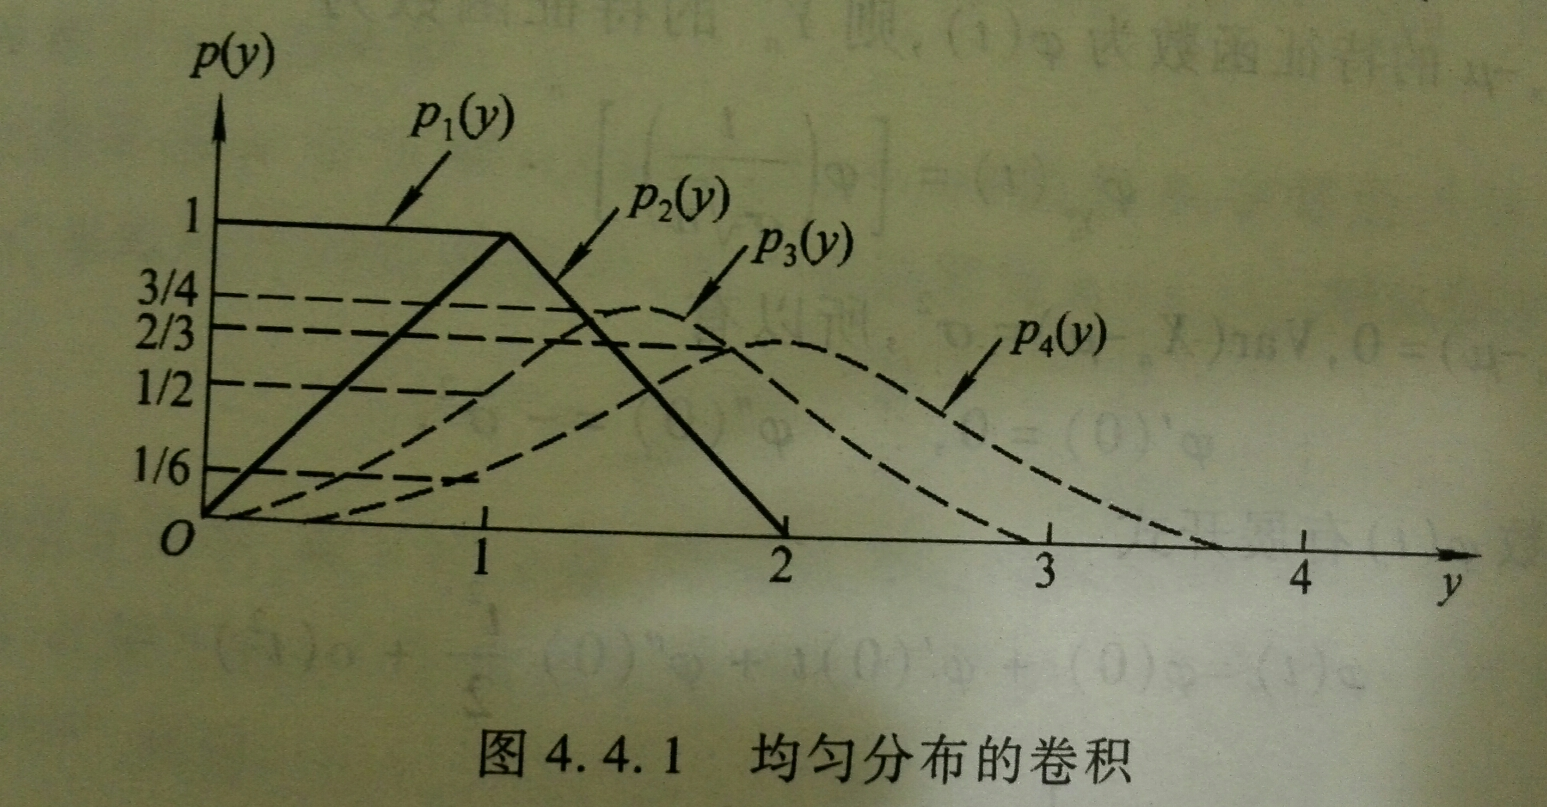
\includegraphics[width=9cm]{uniform.jpg}
	\end{figure}

\end{frame}

\begin{frame}
	\frametitle{问题:寻求 $Y_n$ 的极限分布}
	\begin{itemize}[<+-|alert@+>]
		\item 从上面均匀分布的例子可知:
		\begin{eqnarray*}
			E(Y_n)=\pause \sum_{i=1}^nE(X_i)=\dfrac{n}{2}\rightarrow\infty\\
			D(Y_n)=\pause \sum_{i=1}^n D(X_i)=\dfrac{n}{12}\rightarrow\infty
		\end{eqnarray*}
		\item 考虑 $Y_n$ 的极限分布时,需对 $Y_n$ 进行标准化:
		\begin{eqnarray*}
			Y_n^*:=\dfrac{Y_n-E(Y_n)}{\sqrt{D(Y_n)}}
		\end{eqnarray*}
		\item 在什么情况下
		\begin{eqnarray*}
			\lim_{n\rightarrow\infty}P(Y_n^*\le y)=\dfrac{1}{\sqrt{2\pi}}\int_{-\infty}^ye^{-u^2/2}du
		\end{eqnarray*}

	\end{itemize}
\end{frame}

\begin{frame}
	\frametitle{独立同分布情形下的中心极限定理}
	\begin{thm}[林德伯格 - 莱维 (Lindeberg-L{\'e} vy) 中心极限定理] 设 $\{X_n\}$ 是独立同分布的随机变量序列,且 $E (X_i)=\mu, D (X_i)=\sigma^2>0$ 存在,若记
		\begin{eqnarray*}
			Y_n^*=\dfrac{\sum_{i=1}^nX_i-n\mu}{\sigma\sqrt{n}},
		\end{eqnarray*}
		则对任意的 $y\in R$ 有
		\begin{eqnarray*}
			\lim_{n\rightarrow\infty}P(Y_n^*\le y)=\dfrac{1}{\sqrt{2\pi}}\int_{-\infty}^ye^{-u^2/2}du
		\end{eqnarray*}

	\end{thm}
\end{frame}
\begin{frame}
	\frametitle{Lindeberg-L{\'e}vy 中心极限定理的证明}
	\zheng 要证 $Y_n^*$ 依分布收敛于标准正态分布,只需要说明其特征函数收敛于标准正态分布的特征函数即可. \pause 注意到 $Y_n^*=\sum_{i=1}^n\dfrac{X_i-\mu}{\sigma\sqrt{n}}$. 故若记 $Z_i:=X_i-\mu$ 的特征函数为 $\varphi (t)$, 则
	\begin{eqnarray*}
		\varphi(t)&=&\pause \varphi(0)+\varphi'(0)t+\varphi''(0)\frac{t^2}{2}+o(t^2)\\
		&=&\pause 1+iE(Z_i)+i^2E(Z_i^2)\frac{t^2}{2}+o(t^2)\\
		&=&\pause 1-\frac{\sigma^2t^2}{2}+o(t^2)\\
		\varphi_{Y_n^*}&=&\pause \bigg[\varphi(\frac{t}{\sigma\sqrt{n}})\bigg]^n=\pause \bigg[1-\frac{t^2}{2n}+o(\frac{t^2}{n\sigma^2})\bigg]^n\rightarrow \pause e^{-t^2/2}
	\end{eqnarray*}

\end{frame}
\begin{frame}
	\frametitle{标准正态随机数的产生}
	\begin{itemize}[<+-|alert@+>]
		\item 在随机模拟中经常会需要产生正态随机数,下面我们介绍一种利用中心极限定理通过 $(0,1)$ 上的均匀分布的随机数来产生正态分布 $N (\mu,\sigma^2)$ 随机数的方法;
		\item 中心极限定理理论分析:设 $X_1,\cdots,X_n,\cdots$ 为一列独立同 $(0,1)$ 上的均匀分布的随机变量序列,则 $E (X_i)=1/2, D (X_i)=1/12$, 故
		\begin{eqnarray*}
			\dfrac{\sum_{i=1}^nX_i-n/2}{\sqrt{n/12}}\rightarrow~ \sim N(0,1)
		\end{eqnarray*}
		特别的,若 $n=12$, 则 $X_1+X_2+\cdots+X_{12}-6$ 近似服从标准正态分布.
		\item 产生正态随机数的方法:
		\begin{itemize}
			\item 从计算机中产生 12 个 $(0,1)$ 上均匀分布随机数,记为 $x_1,\cdots, x_{12}$;
			\item 计算 $y=x_1+\cdots+x_{12}-6$, 由上面分析知可将 $y$ 看成 $N (0,1)$ 的一个随机数;
			\item 计算 $z=\mu+\sigma y$, 可将 $z$ 看成 $N (\mu,\sigma^2)$ 分布的随机数;
			\item 重复上面步骤 $n$ 次,即可得到 $n$ 个 $N (\mu,\sigma^2)$ 分布随机数.
		\end{itemize}

	\end{itemize}
\end{frame}
% \begin{frame}
	%   \frametitle{数值计算中的误差分析 I}
	%   \begin{itemize}[<+-|alert@+>]
		%   \item 在数值计算中,任何实数 $x$ 只能通过一定位数的小数 $x'$ 来近似,不妨设我们用四舍五入法得到的 $k$ 位小数来近似;
		%   \item 若 $x'=a_0.a_1a_2\cdots a_k$, 则 $\epsilon:=x-x'\in (-0.5*10^{-k},0.5*10^{-k})$;
		%   \item 考虑一般情形,对于任何实数 $x$, 假设我们通过某种方法选取某个 $k$ 位小数 $x'$ 近似 $x$ 并且假设其误差 $\epsilon$ 服从 $(-0.5*10^{-k},0.5*10^{-k})$ 上的均匀分布 $U (-0.5*10^{-k},0.5*10^{-k})$;
		%   \item 考虑 $n$ 个实数 $x_1,\cdots, x_n$ 的和 $S$ 的近似值 $S'$: 假设 $S$ 中的每一个 $x_i$ 均采用上述一般情形下的近似方法获得其近似值 $x'$, 如果记个别误差为 $\epsilon_i:=x_i-x_i'$, 则总误差为
		%     \begin{eqnarray*}
			%       S-S'=\sum_{i=1}^n(x_i-x_i')=\sum_{i=1}^n\epsilon_i
			%     \end{eqnarray*}
		%   \item 根所假设,我们可以认为 $\epsilon_i\sim U (-0.5*10^{-k},0.5*10^{-k})$, 且相互独立.
		%   \end{itemize}
	% \end{frame}
% \begin{frame}
	%   \begin{columns}
		%     \column{5cm}
		%     \begin{figure}
			%       \centering
			%       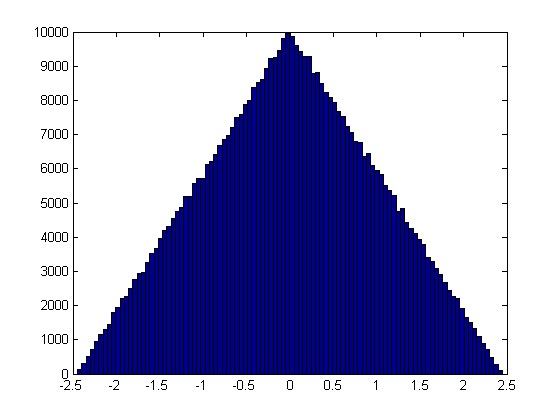
\includegraphics[width=5cm]{2sumuniform.png}
			%     \end{figure}
		%     \column{5cm}
		%     \begin{figure}
			%       \centering
			%       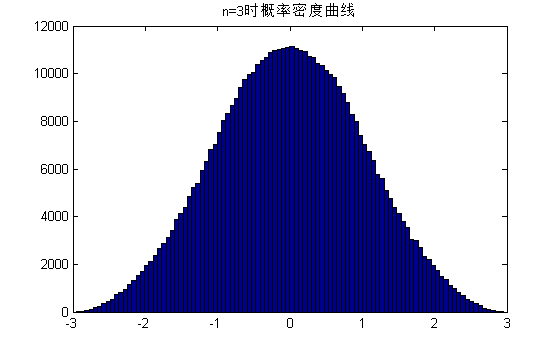
\includegraphics[width=5cm]{3sumuniform.png}
			%     \end{figure}

		%   \end{columns}
	%   \begin{columns}
		%     \column{5cm}
		%     \begin{figure}
			%       \centering
			%       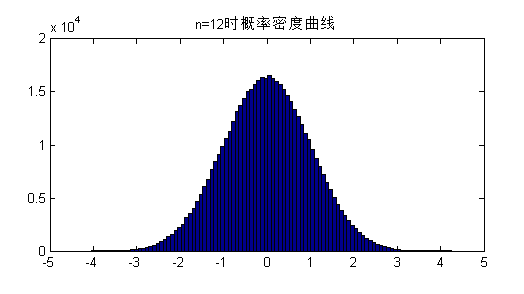
\includegraphics[width=5cm]{12sumuniform1.png}
			%     \end{figure}
		%     \column{5cm}
		%     \begin{figure}
			%       \centering
			%       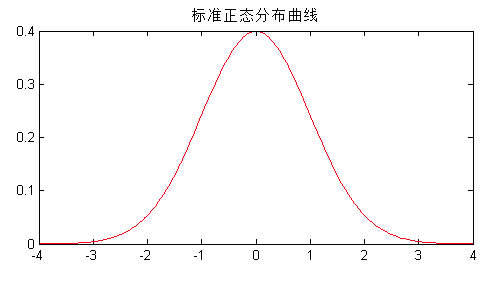
\includegraphics[width=5cm]{n01.png}
			%     \end{figure}

		%   \end{columns}
	% \end{frame}
% \begin{frame}
	%   \frametitle{数值计算中的误差分析 II}
	%   \begin{itemize}[<+-|alert@+>]
		%   \item 一种粗略的估计总误差的方法为:由于 $|\epsilon_i|\le 0.5*10^{-k}$, 故
		%     \begin{eqnarray*}
			%       |\sum_{i=1}^n\epsilon_i|\le n*0.5*10^{-k}
			%     \end{eqnarray*}
		%   \item 利用中心极限定理: $\epsilon_i$ 独立同分布且 $E (\epsilon_i)=0,D (\epsilon_i)=\dfrac{10^{-2k}}{12}$, 故
		%{\small\begin{eqnarray*}
				%              P(\sum_{i=1}^n\epsilon_i|\le z)&=&\pause P(\bigg|\dfrac{\sum_{i=1}^n\epsilon_i-0}{\sqrt{n10^{-2k}/12}}\bigg|\le \dfrac{z}{\sqrt{n10^{-2k}/12}})\\
				%                                             &\approx&\pause \Phi(\dfrac{z}{\sqrt{n10^{-2k}/12}})-\Phi(-\dfrac{z}{\sqrt{n10^{-2k}/12}})\\
				%                                             &=&\pause 2\Phi(\dfrac{z}{\sqrt{n10^{-2k}/12}})-1
				%            \end{eqnarray*}}
		%        \item 若令上面的概率为 $0.99$, 则 $\Phi (\dfrac{z}{\sqrt{n10^{-2k}/12}})=0.995$, 反查正态分布函数表可得 \vspace{-0.7cm}
		%          \begin{eqnarray*}
			%            \hspace{1.2cm} \dfrac{z}{\sqrt{n10^{-2k}/12}}=2.576\Rightarrow z=2.576\sqrt{n10^{-2k}/12}
			%          \end{eqnarray*}

		%        \end{itemize}


	%      \end{frame}

\begin{frame}
	\frametitle{二项分布的正态近似}
	\begin{thm}[棣莫弗 - 拉普拉斯中心极限定理] 设 $n$ 重伯努利试验中,事件 $A$ 在每次试验中出现的概率为 $p\in (0,1)$, 记 $S_n$ 为 $n$ 重伯努利试验中事件 $A$ 出现的次数,则对任意的 $y\in R$ 均有
		\begin{eqnarray*}
			\lim_{n\rightarrow\infty}P(\dfrac{S_n-np}{\sqrt{np(1-p)}}\le y)=\dfrac{1}{\sqrt{2\pi}}\int_{-\infty}^ye^{-u^2/2}du
		\end{eqnarray*}

	\end{thm}
	\pause 在上述定理中,若记 $\Phi (y)=\beta, Y_n^*:=\dfrac{S_n-np}{\sqrt{np (1-p)}}$, 则
	\begin{eqnarray*}
		P(Y_n^*\le y)\approx \Phi(y)=\beta
	\end{eqnarray*}


\end{frame}

% \begin{frame}
	%   \frametitle{二项分布正态近似的几点注意}
	%   \begin{itemize}[<+-|alert@+>]
		%   \item 与二项分布的泊松近似相比:一般来说,$p$ 较小时,用泊松分布近似较好;而在 $np>5$ 和 $n (1-p)>5$ 时,正态分布近似较好;
		%   \item 因二项分布是离散分布,正态分布是连续分布,故用正态分布近似时,作些修正可以提高精度:若 $k_1<k_2$, 一般先作如下修正再用正态近似 $P (k_1\le S_n\le k_2)=P (k_1-0.5<S_n<k_2-0.5)$;
		%   \item 对于二项分布的计算,用修正的正态近似还可得
		%     \begin{eqnarray*}
			%       P(S_n=k)&=&\pause P(k-0.5<S_n<k+0.5)\\
			%               &=&\pause P(\dfrac{k-0.5-np}{\sqrt{np(1-p)}}<\dfrac{S_n-np}{\sqrt{np(1-p)}}<\dfrac{k+0.5-np}{\sqrt{np(1-p)}})\\
			%               &\approx&\pause\int_{\frac{k-0.5-np}{\sqrt{np(1-p)}}}^{\frac{k+0.5-np}{\sqrt{np(1-p)}}} \dfrac{1}{\sqrt{2\pi}}e^{-x^2/2}dx\\
			%               &\approx&\pause \dfrac{1}{\sqrt{2\pi}}e^{-(\frac{k-np}{\sqrt{np(1-p)}})^2/2}\cdot \dfrac{1}{\sqrt{np(1-p)}}
			%     \end{eqnarray*}

		%   \end{itemize}

	% \end{frame}
\begin{frame}
	\frametitle{独立不同分布下的中心极限定理}
	\begin{itemize}[<+-|alert@+>]
		\item 设 $\{X_n\}$ 是一个相互独立的随机变量序列,其期望与方差有限分别为
		\begin{eqnarray*}
			E(X_i)=\mu_i, \quad D(X_i)=\sigma_i^2, \quad i=1,2,\cdots,
		\end{eqnarray*}
		\item 考虑随机变量的和 $\textcolor{red}{Y_n=X_1+\cdots+X_n}$, 则
		\begin{eqnarray*}
			E(Y_n)=\mu_1+\cdots+\mu_n,\quad \textcolor{red}{\sigma(Y_n):=\sqrt{D(Y_n)}=\sqrt{\sigma_1^2+\cdots+\sigma_n^2}}
		\end{eqnarray*}
		\item 考虑 $Y_n$ 的标准化:$ Y_n^*:=\dfrac{Y_n-E (Y_n)}{\sigma (Y_n)}=\sum_{i=1}^n\dfrac{X_i-\mu_i}{\sigma (Y_n)}$
		\item 要求 $Y_n^*$ 中的各项 $\dfrac{X_i-\mu_i}{\sigma (Y_n)}$ 均匀的小,即对任意的 $\tau>0$, 要求事件
		\begin{eqnarray*}
			A_{ni}=\left\{\dfrac{X_i-\mu_i}{\sigma(Y_n)}>\tau\right\}=\left\{|X_i-\mu_i|>\tau\sigma(Y_n)\right\}
		\end{eqnarray*}
		发生的可能性小或直接要求其概率趋于 0.
		\item 为达目的,我们要求 $\lim_{n\rightarrow\infty} P (\max_{1\le i\le n}|X_i-\mu_i|>\tau\sigma (Y_n))=0$
	\end{itemize}
\end{frame}
\begin{frame}
	\frametitle{$\lim_{n\rightarrow\infty}P(\max_{1\le i\le n}|X_i-\mu_i|>\tau\sigma(Y_n))=0$}
	注意到
	\begin{eqnarray*}
		&&P(\max_{1\le i\le n}|X_i-\mu_i|>\tau\sigma(Y_n))=\pause P(\cup_{i=1}^n|X_i-\mu_i|>\tau\sigma(Y_n))\\
		&&\le\pause \sum_{i=1}^nP(|X_i-\mu_i|>\tau\sigma(Y_n))=\pause \sum_{i=1}^n\int_{|x-\mu_i|>\tau\sigma(Y_n)}dF_i(x)\\
		&&\le \pause \dfrac{1}{\tau^2\sigma(Y_n)^2}\sum_{i=1}^n\int_{|x-\mu_i|>\tau\sigma(Y_n)}(x-\mu_i)^2dF_i(x)
	\end{eqnarray*}

	\pause 故只要下面的 \textcolor{red}{\bf 林德伯格条件} 满足
	\begin{eqnarray*}%\label{eq:Lindeberg}
		\lim_{n\rightarrow\infty} \dfrac{1}{\tau^2\sigma(Y_n)^2}\sum_{i=1}^n\int_{|x-\mu_i|>\tau\sigma(Y_n)}(x-\mu_i)^2dF_i(x)=0
	\end{eqnarray*}
	就可保证 $Y_n^*$ 中各加项充分的小


\end{frame}

\begin{frame}
	\frametitle{林德伯格中心极限定理}
	\begin{thm}
		设独立随机变量序列 $\{X_n\}$ 满足林德伯格条件
		\begin{eqnarray}\label{eq:Lindeberg}
			\lim_{n\rightarrow\infty} \dfrac{1}{\tau^2\sigma(Y_n)^2}\sum_{i=1}^n\int_{|x-\mu_i|>\tau\sigma(Y_n)}(x-\mu_i)^2dF_i(x)=0
		\end{eqnarray} 则对任意的 $x$, 有
		\begin{eqnarray*}
			\lim_{n\rightarrow\infty}P(\dfrac{1}{\sigma(Y_n)}\sum_{i=1}^n(X_i-\mu_i)\le x)=\dfrac{1}{\sqrt{2\pi}}\int_{-\infty}^xe^{-u^2/2}du
		\end{eqnarray*}
	\end{thm}
	\pause
	\begin{rmk}
		假设 $\{X_n\}$ 独立同分布且方差有限,则容易验证上述的林德伯格条件满足,从而我们先前在独立同分布情形下的中心极限定理是林德伯格中收极限定理的特例.
	\end{rmk}
\end{frame}

\begin{frame}{一个引理}
	\begin{lem}\label{lem:eixtaylor}
		对一切 $x \in R$ 及非负整数 $n$ 有
		\[
		\left|e^{i x}-\sum_{k=0}^{n} \frac{(i x)^{k}}{k!}\right| \leq\left[\frac{|x|^{n+1}}{(n+1)!}\right] \wedge\left[\frac{2|x|^{n}}{n!}\right]
		\]
	\end{lem}

\end{frame}
\begin{frame}{引理证明}
\begin{itemize}
	\item 用分部积分可得
	\begin{align}\label{eq:sepinte}
		\int_{0}^{x}(x-s)^{n} e^{i s} d s=\frac{x^{n+1}}{n+1}+\frac{i}{n+1} \int_{0}^{x}(x-s)^{n+1} e^{i s} d s
	\end{align}

	\item 递归可得知,对一切 $n \geq 0$ 有
	\begin{align}\label{eq:digui}
		e^{i x}=\sum_{k=0}^{n} \frac{(i x)^{k}}{k!}+\frac{i^{n+1}}{n!} \int_{0}^{x}(x-s)^{n} e^{i s} d s
	\end{align}

	\item
	由此推出估计式$
	\big|e^{i x}-\sum_{k=0}^{n} \dfrac{(i x)^{k}}{k!}\big| \leq \dfrac{|x|^{n+1}}{(n+1)!}$
	\item 将\eqref{eq:sepinte}式中 $n$ 换为 $n-1$ ,解出右方积分并代入\eqref{eq:digui}便推出
	\[
	e^{i x}=\sum_{k=0}^{n} \frac{(i x)^{k}}{k!}+\frac{i^{n}}{(n-1)!} \int_{0}^{x}(x-s)^{n-1}\left(e^{i s}-1\right) d s
	\]
\item 故可得另一估计式$
	\left|e^{i x}-\sum_{k=0}^{n} \dfrac{(i x)^{k}}{k!}\right| \leq \dfrac{2|x|^{n}}{n!}$
\item 联合上述两个估计式可得引理结论.%(4.10)与(4.11)便得到(4.7)式,引理证完。


\end{itemize}

\end{frame}
\begin{frame}{引理的几个常用结论}
\begin{rmk} 若引理中的$n=0,1,2$, 则有%的特例以备引用:
	\begin{align*}
		\left|e^{i x}-1\right| & \leq|x| \wedge 2 \\
		\left|e^{i x}-1-i x\right| & \leq \frac{x^{2}}{2} \wedge(2|x|) \\
		\left|e^{i x}-1-i x+\frac{x^{2}}{2}\right| & \leq\left(\frac{1}{6}|x|^{3}\right) \wedge x^{2}
	\end{align*}
\end{rmk}

\end{frame}

\begin{frame}{林德伯格中心极限定理证明}
\begin{itemize}
	\item 只需证 $Y_n^*:=\frac{\sum_{k=1}^n(X_k-E[X_k])}{\sqrt{D(\sum_{k=1}^nX_k)}}$ 的特征函数列收敛到标准正态分布的特征函数,即
	\begin{align}\label{eq:celimit}
		\lim_{n\rightarrow\infty}\phi_{n}(t)=\lim_{n\rightarrow\infty}E[e^{itY_n^*}]= \exp\{-\frac{t^2}{2}\}.
	\end{align}

    \item 对一切 $n \geq 1$ 及 $k=1, \cdots, n$,令 $X_{nk}=\left(X_{k}-\mu_k\right) / \sigma(Y_n)$, 则
	\[E\left(X_{nk}\right)=0,\quad D\left(X_{nk}\right)=\sigma_k^{2} / \sigma(Y_n)^{2}.\]
	\item 以 $F_{n k}(x)$ 及 $\phi_{n k}(t)$ 分别表 $X_{nk}$的分布函数及特征函数.
		\item 已知的林德伯格条件\eqref{eq:Lindeberg}式化为
		\begin{align}\label{eq:Lindebergcondi-2}
			\lim _{n} \sum_{k=1}^{n} \int_{(|x| \geq \tau)} x^{2} d F_{n k}(x)=0, \ \forall \tau>0
		\end{align}

	\item
		而待证的\eqref{eq:celimit}式变为 $n \rightarrow \infty$ 时有
		\[
		\phi_{n}(t)=\prod_{k=1}^{n} \phi_{n k}(t) \longrightarrow \exp\{-\frac{t^2}{2}\},  \forall t \in R
		\]

\end{itemize}

\end{frame}
\begin{frame}{林德伯格中心极限定理证明}
	\begin{itemize}
		\item 注意到
		\begin{align*}
		  \phi_{nk}(t)&\approx 1+\phi_{nk}'(0)t+\frac{1}{2}\phi_{nk}''(0)t^2=1+iE[X_{nk}]t+\frac{1}{2}i^2E[X_{nk}^2]t^2\\
					&=1-\frac{t^2\sigma_k^2}{2\sigma(Y_n)^2}\approx \exp\{-\frac{t^2\sigma_k^2}{2\sigma(Y_n)^2}\}\\
			\exp\{-\frac{t^2}{2}\}&=\exp\{-\frac{t^2}{2}\sum_{k=1}^n\frac{\sigma_k^2}{\sigma(Y_n)^2}\}=\prod_{k=1}^{n} \exp\{-\frac{t^2\sigma_k^2}{2\sigma(Y_n)^2}\}
		\end{align*}
		\item 因此,欲证$\phi_{n}(t)=\prod_{k=1}^{n} \phi_{n k}(t) \longrightarrow e^{-\frac{t^{2}}{2}},  \forall t \in R$, 只需证明
		\begin{align*}
	&\big|\prod_{k=1}^{n} \phi_{n k}(t)-\prod_{k=1}^{n}\big(1-\frac{t^{2} \sigma_{k}^{2}}{2 \sigma(Y_n)^2}\big)\big| \longrightarrow 0\\
	&\big|\prod_{k=1}^{n}\big(1-\frac{t^{2} \sigma_{k}^{2}}{2 \sigma(Y_n)^2}\big)-\prod_{k=1}^{n} \exp\{-\frac{t^2\sigma_k^2}{2\sigma(Y_n)^2}\}\big| \longrightarrow 0
		\end{align*}
	\end{itemize}


	\end{frame}
	\begin{frame}{证明:$\big|\prod_{k=1}^{n} \phi_{n k}(t)-\prod_{k=1}^{n}\big(1-\frac{t^{2} \sigma_{k}^{2}}{2 \sigma(Y_n)^2}\big)\big| \rightarrow 0$}
		\vspace{-0.1cm}
		\begin{itemize}
			\item 由引理\ref{lem:eixtaylor}可知,对一切 $t \in R$ 有
		\[
		\big|e^{i t x}-\big(1+i t x-\frac{1}{2} t^{2} x^{2}\big)\big| \leq|t x|^{2} \wedge|t x|^{3}
		\]
		\item 注意到 $X_{nk}$ 二阶矩有限,两边对 $F_{n k}$ 取积分得
		\[
		\big|\phi_{n k}(t)-\big(1-\frac{t^{2} \sigma_{k}^{2}}{2 \sigma(Y_n)^{2}}\big)\big| \leq E\big\{\big|t X_{nk}\big|^{2} \wedge\big|t X_{nk}\big|^{3}\big\}
		\]
		\item 而对任何 $\tau>0$ ,上式右方不超过
		\begin{align*}
			&\int_{(|x|<\tau)}|t x|^{3} d F_{n k}(x)+\int_{(|x| \geq \tau)}(t x)^{2} d F_{n k}(x)\\
			&\leq \tau|t|^{3} \frac{\sigma_{k}^{2}}{\sigma(Y_n)^{2}}+t^{2} \int_{(|x| \geq \tau)} x^{2} d F_{n k}(x)
		\end{align*}
		\item 由于 $\sum_{k=1}^{n} \sigma_{k}^{2} / \sigma(Y_n)^{2}=D\big(Y_n^*\big)=1$, 求和便推出
		\[
		\sum_{k=1}^{n}\big|\phi_{n k}(t)-\big(1-\frac{t^{2} \sigma_{k}^{2}}{2 \sigma(Y_n)^{2}}\big)\big| \leq \tau|t|^{3}+t^{2} \sum_{k=1}^{n} \int_{(|x| \geq \tau)} x^{2} d F_{n k}(x)
		\]
		\end{itemize}
	\end{frame}

	\begin{frame}{证明:$\big|\prod_{k=1}^{n} \phi_{n k}(t)-\prod_{k=1}^{n}\big(1-\frac{t^{2} \sigma_{k}^{2}}{2 \sigma(Y_n)^2}\big)\big| \rightarrow 0$}
\begin{itemize}
	\item 上式先令 $n \rightarrow \infty$ 再令 $\tau \downarrow 0$, 由\eqref{eq:Lindebergcondi-2}式得
	\[
	\sum_{k=1}^{n}\big|\phi_{n k}(t)-\big(1-\frac{t^{2} \sigma_{k}^{2}}{2 \sigma(Y_n)^2}\big)\big| \rightarrow 0,  t \in R
	\]
	\item 故
	\begin{align*}
		\big|\prod_{k=1}^{n} \phi_{n k}(t)-\prod_{k=1}^{n}\big(1-\frac{t^{2} \sigma_{k}^{2}}{2 \sigma(Y_n)^2}\big)\big|\leq  \sum_{k=1}^{n}\big|\phi_{n k}(t)-\big(1-\frac{t^{2} \sigma_{k}^{2}}{2 \sigma(Y_n)^2}\big)\big| \rightarrow 0
	\end{align*}得证.
\end{itemize}
	\end{frame}

\begin{frame}{证明:$\big|\prod_{k=1}^{n}\big(1-\frac{t^{2} \sigma_{k}^{2}}{2 \sigma(Y_n)^2}\big)-\prod_{k=1}^{n} \exp\{-\frac{t^2\sigma_k^2}{2\sigma(Y_n)^2}\}\big| \rightarrow 0$}
\vspace{-0.1cm}
\begin{itemize}

	\item 注意到当 $|z| \leq 1 / 2$ 时有
	{\small \[
	\left|e^{z}-1-z\right| \leq \frac{1}{2} \sum_{k=2}^{\infty}|z|^{k}=\frac{1}{2}|z|^{2} /(1-|z|) \leq z^{2}
	\]}
    \item 取 $z=\frac{t^{2} \sigma_{k}^{2}}{2 \sigma(Y_n)^2}$, 可得
    {\small \begin{align*}
		&\big|\prod_{k=1}^{n}\big(1-\frac{t^{2} \sigma_{k}^{2}}{2 \sigma(Y_n)^2}\big)-\prod_{k=1}^{n} \exp\{-\frac{t^2\sigma_k^2}{2\sigma(Y_n)^2}\}\big|\\
		&\leq \sum_{k=1}^{n}\big|\exp\{-\frac{t^2\sigma_k^2}{2\sigma(Y_n)^2}\}-\big(1-\frac{t^{2} \sigma_{k}^{2}}{2 \sigma(Y_n)^2}\big)\big|\\
		&\leq \frac{t^4}{4}\sum_{k=1}^{n}\big(\frac{\sigma_{k}^{2}}{\sigma(Y_n)^2}\big)^2\leq \frac{t^{4}}{4}\left(\max _{1 \leq k \leq n} \frac{\sigma_{k}^{2}}{\sigma(Y_n)^2}\right) \sum_{k=1}^{n} \frac{\sigma_{k}^{2}}{\sigma(Y_n)^2}\\
		&\leq \frac{t^{4}}{4}\left(\max _{1 \leq k \leq n} \frac{\sigma_{k}^{2}}{\sigma(Y_n)^2}\right)
	\end{align*}}
	\item 若$\max _{1 \leq k \leq n} \frac{\sigma_{k}^{2}}{\sigma(Y_n)^2}\rightarrow 0$, 则定理得证.
\end{itemize}

\end{frame}


\begin{frame}{证明: $\max _{1 \leq k \leq n} \frac{\sigma_{k}^{2}}{\sigma(Y_n)^2}\rightarrow 0$}
	\vspace{-0.1cm}
\begin{itemize}
	\item 对任何 $\tau>0$ 有
\begin{align*}
	\frac{\sigma_{k}^{2}}{\sigma(Y_n)^2}=D\left(X_{n k}\right)&=\int_{-\infty}^{+\infty}x^2dF_{nk}(x)\\
	&=\int_{|x|<\tau}x^2dF_{nk}(x)+\int_{|x|\geq\tau}x^2dF_{nk}(x)\\
	&\leq \tau^{2}+\int_{(|x| \geq \tau)} x^{2} d F_{n k}(x)
\end{align*}
\item 从而
	\[
	\max _{1 \leq k \leq n} \frac{\sigma_{k}^{2}}{\sigma(Y_n)^2} \leq \tau^{2}+\sum_{k=1}^{n} \int_{(|x| \geq \tau)} x^{2} d F_{n k}(x)
	\]
\item
	再次令 $n \rightarrow \infty$ 及 $\tau \downarrow 0$, 由\eqref{eq:Lindebergcondi-2}式得
	\[
	\lim _{n}\left\{\max _{1 \leq k \leq n} \frac{\sigma_{k}^{2}}{\sigma(Y_n)^2}\right\}=0
	\]
	\item 进而, 若$z=\frac{t^{2} \sigma_{k}^{2}}{2 \sigma(Y_n)^2}$, 当$n$充分大时$|z| \leq 1 / 2$.
\end{itemize}

\end{frame}








\begin{frame}
	\frametitle{推出 Lindeberg 条件的充分条件}
	\begin{thm}
		设 $\{X_n\}$ 为独立随机变量序列,如果存在常数列 $\{L_n\}$ 使得
		\begin{eqnarray*}
			\max_{1\leq k\leq n}|X_k|\leq L_n, \mbox{ 且 } \lim_{n}\dfrac{L_n}{\sigma(Y_n)}=0
		\end{eqnarray*}
		则 Lindeberg 条件成立,从而 $\{X_n\}$ 满足中心极限定理.
	\end{thm}

\zheng
\begin{itemize}
	\item 由假设知,对于 $\tau>0$ ,存在 $N$ ,使当 $n \geq N$ 时有 $2 L_{n}<$ $\tau \sigma(Y_n)$.
	\item 因此当 $n \geq N$ 时对一切 $k=1, \cdots, n$ 有 $\Omega=\left\{\left|X_{k}-\mu_{k}\right|<\tau \sigma(Y_n)\right\}$.
	\item 故 $n \geq N$ 时有
	\begin{align*}
		&\frac{1}{\sigma(Y_n)^{2}} \sum_{k=1}^{n} \int_{\left(\left|x-\mu_{k}\right|<\tau \sigma(Y_n)\right)}\left(x-\mu_{k}\right)^{2} d F_{k}(x)\\
		&=\frac{1}{\sigma(Y_n)^{2}} \sum_{k=1}^{n} \int_{-\infty}^\infty\left(x-\mu_{k}\right)^{2} d F_{k}(x)=1 .
	\end{align*}
\item 这表明林德伯格条件\eqref{eq:Lindeberg} 式成立,故 $\left\{X_{n}\right\}$ 满足中心极限定理.
\end{itemize}




\end{frame}

\begin{frame}
	\frametitle{李雅普诺夫中心极限定理}
	\begin{thm} 设 $\{X_n\}$ 为独立随机变量序列,若存在 $\delta>0$ 满足
		\begin{eqnarray*}
			\lim_{n\rightarrow\infty}\dfrac{1}{\sigma(Y_n)^{2+\delta}}\sum_{k=1}^nE(|X_k-\mu_k|^{2+\delta})=0,
		\end{eqnarray*}
		则 $\lim_{n\rightarrow\infty}P(\dfrac{1}{\sigma(Y_n)}\sum_{k=1}^n(X_k-\mu_k)\le x)=\dfrac{1}{\sqrt{2\pi}}\int_{-\infty}^xe^{-u^2/2}du$.
		% \begin{eqnarray*}
		% 	\lim_{n\rightarrow\infty}P(\dfrac{1}{\sigma(Y_n)}\sum_{i=1}^n(X_i-\mu_i)\le x)=\dfrac{1}{\sqrt{2\pi}}\int_{-\infty}^xe^{-u^2/2}du
		% \end{eqnarray*}

	\end{thm}

	\zheng 只要验证林德伯格条件成立. 实际上对任何 $\tau>0$ 有
	\begin{align*}
		& \lim _{n} \frac{1}{\sigma(Y_n)^{2}} \sum_{k=1}^{n} \int_{\left(\left|x-\mu_k\right| \geq \tau \sigma(Y_n)\right)}\left(x-\mu_{k}\right)^{2} d F_{k}(x) \\
		\leq & \lim _{n} \frac{1}{\sigma(Y_n)^{2}\left(\tau \sigma(Y_n)\right)^{\delta}} \sum_{k=1}^{n} \int_{\left(\left|x-\mu_k\right| \geq \tau \sigma(Y_n)\right)}\left|x-\mu_k\right|^{2+\delta} d F_{k}(x) \\
		\leq & \lim _{n} \frac{1}{\tau^{\delta}} \frac{1}{\sigma(Y_n)^{2+\delta}} \sum_{k=1}^{n} \int_{\Re}\left|x-\mu_{k}\right|^{2+\delta} d F_{k}(x)=0 .
	\end{align*}
	定理证毕.
\end{frame}








